%\documentclass[handout]{beamer}
\documentclass[presentation]{beamer}

\usecolortheme{UTUaaro}
 
\usepackage[utf8]{inputenc}
\usepackage[UKenglish]{babel}
\usepackage{booktabs}
\usepackage{caption}
\usepackage{subcaption}
\usepackage{graphicx}
\usepackage{amsmath}
\usepackage{amsfonts}
\usepackage{amssymb}
\usepackage{fancybox}
\usepackage{epstopdf}
\usepackage{hyperref}
\usepackage{pdfpc-commands}

\usepackage{lipsum} % for template demonstration

% complying UK date format, i.e. 1 January 2001
\usepackage{datetime}
\let\dateUKenglish\relax
\newdateformat{dateUKenglish}{\THEDAY~\monthname[\THEMONTH] \THEYEAR}


\institute{
\includegraphics[height=1.5cm]{UTU_logo_RGB_EN.pdf}}


% -----------------------------------------------------------------------------
% vähän tekstiä per slide, paljon yleistajuisia pointteja

% pointeja:
% tilastollinen koneoppisen teemoja:
% paljon samanlaisia yksinkertaisia palasia pystyvät mallintamaan monimutkaisia asioita
% tilatotieteellinen päättely automatisoituna?
%
% ei ihmis- tai eläinkognition/älyn mallintamista, ainakaan kovin usein
% -> neuroverkotkin lähinnä inspiroituneita kuin edes abstrakteja malleja aivokuoresta
%

% tapausesimerkki: % https://www.helsinki.fi/fi/uutiset/terveys/suomalaistutkijat-kehittivat-tekoalyalgoritmin-aivovammapotilaiden-tehohoitoon

% aiheet
% 1. logistinen regressio? muurahainen.
% 2. neuroverkko. limasieni? termiittikeko.

% Aikatauluts + kalvot
% johdanto: 5 min
%   Tekoälystä puhutaan paljon. Ehkä joskus jossain on jotain, mutta minun puhun
%       algoritmeista 
%
%   mitä tilastollinen oppiminen tarkoittaa:
%       
%   kuinka algoritmin onnistumista mitataan
% lineaarinen regressio: 10 min
% logistinen regressio: 10 min
% konvolutiivinen neuroverkko: 10 min
% (päätöspuu -> satunnaismetsät: 10 min)
% yhteenveto: 5 min
% https://link.springer.com/article/10.3758%2Fs13420-020-00410-z
% = 40 min

% laskuesimerkkien toteutus
% optio 1: toteuta Julialla (opin Juliaa!)
% optio 2 jos feilaa: Python ja scikit (kertaan Python-Scikit!)

% https://github.com/bensadeghi/DecisionTree.jl
% https://github.com/JuliaStats/GLM.jl
% https://github.com/FluxML/model-zoo/
% jas nns, also alternative logres. https://github.com/FluxML/model-zoo/blob/master/other/iris/iris.jl

\title{Kurkistus tilastollisesti oppivien koneiden eläintarhaan}

% tavoitemitta: 30-45 min + keskustelu = 15-20 sisältöslidea plus ekstrat
\subtitle{Studia Varjomafia 4, Terrakoti}

\author{Aaro Salosensaari aaro.salosensaari@utu.fi. CC-BY-SA 4.0, paitsi fair use.}

\date{22.2.2020}

\begin{document}
 
\frame{\titlepage}

\section{Eläintarhan portti}


\begin{frame}{}
  \tableofcontents[currentsection]
\end{frame}

\begin{frame}{Mikä on tilastollisesti oppiva kone?}

	\begin{columns}[]
		\column{0.0125\textwidth}
		\column{0.4875\textwidth}
			\centering
			    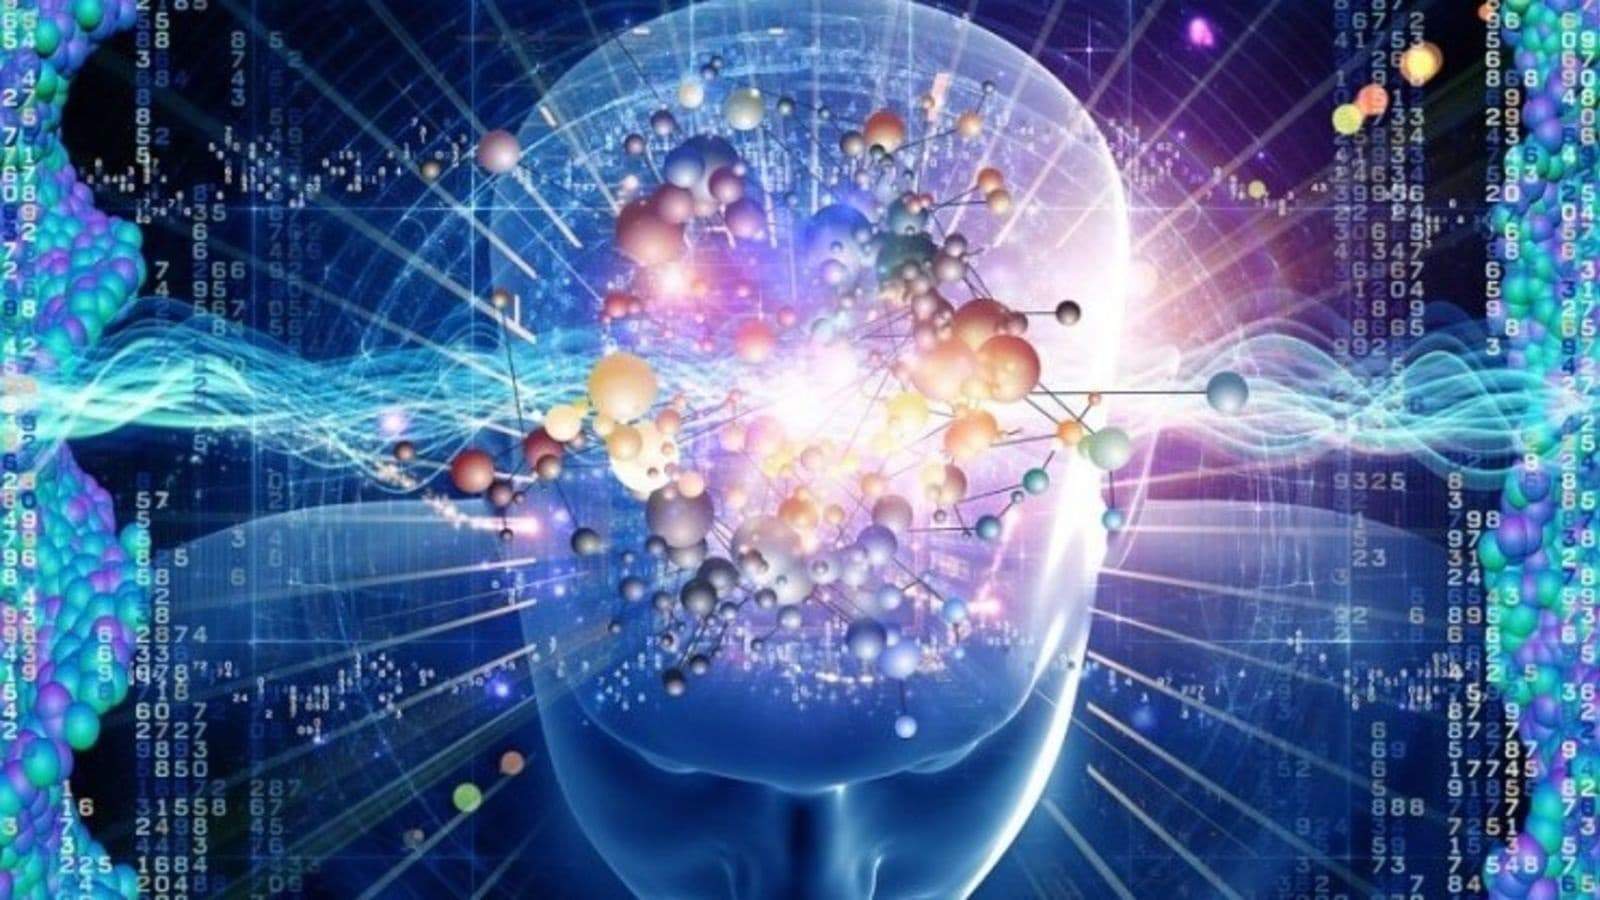
\includegraphics[width=\textwidth]{galaxy-brain-meme.jpg}
		\column{0.4875\textwidth}
		    \centering
		    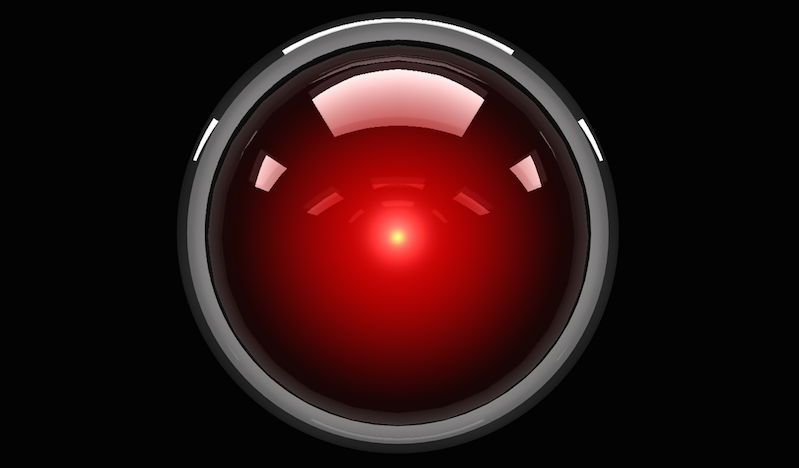
\includegraphics[width=\textwidth]{hal9000.png}
		\column{0.0125\textwidth}
	\end{columns}
    
\end{frame}

\begin{frame}{Tilastollisesti oppiva kone on ... ?}

    Eräs epätarkasti yksinkertaistettu määritelmä:
    
    \begin{block}{Tilastollinen koneoppimisalgoritmi}
    Algoritmi, joka oppii aineistosta ("data") antamaan vastauksia jotka todennäköisesti ($=$ tilastollisesti keskimäärin) ovat oikein.
    \end{block}
    
    \pause
    Seuraava kysymys: Mitä tarkoittaa oppiminen?
\end{frame}

\begin{frame}{Algoritmi joka ei opi}
	\begin{columns}[]
		\column{0.0125\textwidth}
		\column{0.4875\textwidth}
			\centering
			\begin{figure}
				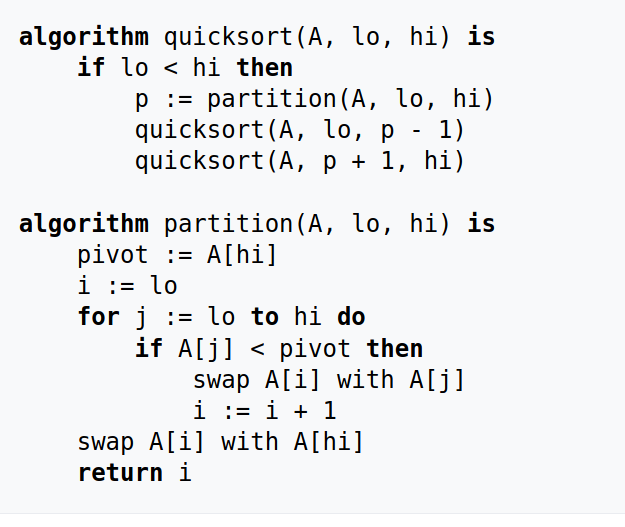
\includegraphics[width=\textwidth]{quicksort.png} \
				% remove the 'draft' keyword, when replacing with final figure!
				% \inlineMovie[loop&autostart&start=5&stop=12]{apollo17.avi}{apollo17.jpg}{height=0.7\textheight}
				\caption*{Quicksort-algoritmi järjestää lukuja askel askeleelta, ja antaa todistettavasti oikean ratkaisun jokaiselle lukujonolle.}
			\end{figure}
		\column{0.4875\textwidth}
		    \centering
		    \begin{figure}
		        \inlineMovie[loop&autostart]{msortin.avi}{sorting_gif-0.png}{width=\textwidth}
		        \caption*{Kuvalähde: Wikipedia User:RolandH CC-BY-SA 3.0 [1] }
		    \end{figure}
		\column{0.0125\textwidth}
	\end{columns}
\end{frame}

\begin{frame}{Algoritmit jotka oppivat}
    
    Algoritmi (ihmisen koodaama ohjelmakoodi) ei ratkaise ongelmaa itsessään (vrt. edel. kalvon quicksort).
    %
    \pause
    
    Sen sijaan ns. oppiva algoritmi koostuu usein oikeastaan kahdesta osasta:
    \pause
    \begin{enumerate}
        \item Malli (jossa on parametreja).
        \item Algoritmi, joka kertoo kuinka valitaan eli \textbf{opitaan} parametrit joilla malli antaa (tilastollisesti keskimäärin) ratkaisuja johonkin \mathbf{tiettyyn} ongelmaan.
    \end{enumerate}
    \pause
    	\begin{columns}[]
		\column{0.0100\textwidth}
		\column{0.4875\textwidth}
			\centering
				
\includegraphics[width=0.6\textwidth]{lasse.jpg}
	    \column{0.005\textwidth}
	        vs.
		\column{0.4875\textwidth}
		    \centering
				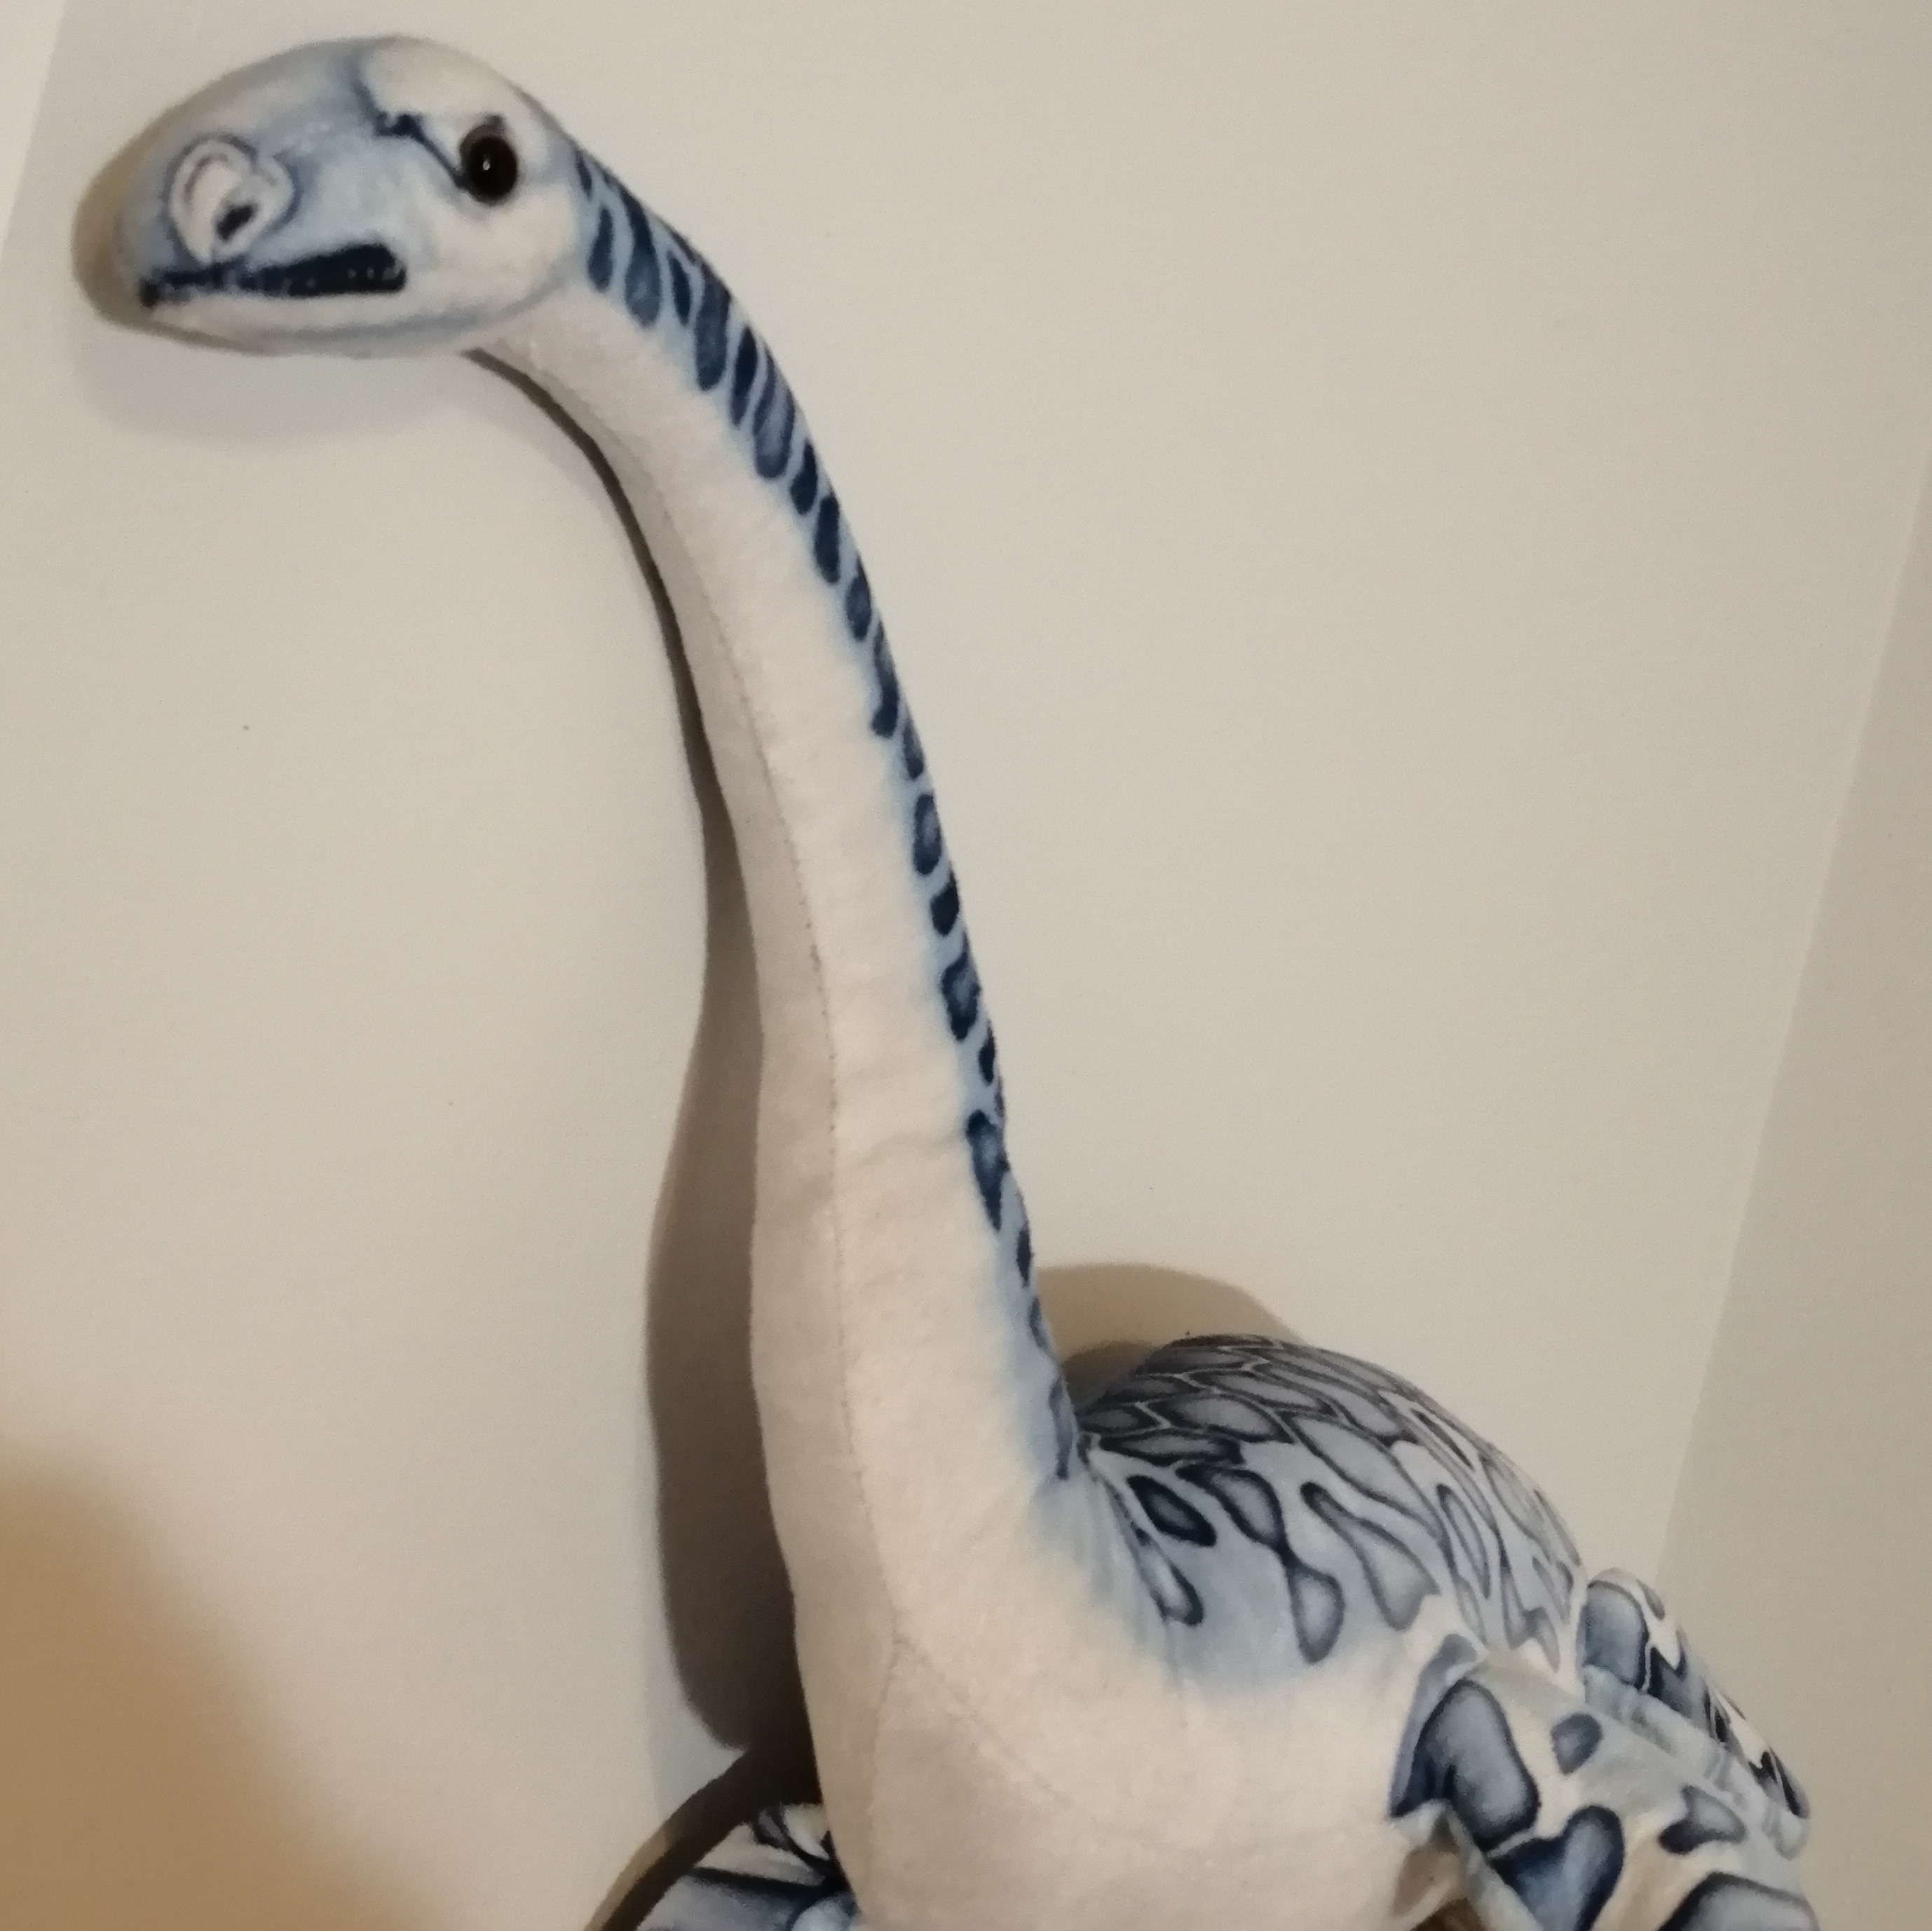
\includegraphics[width=0.6\textwidth]{nessie.jpg}

		\column{0.0100\textwidth}
	\end{columns}
    
\end{frame}

\begin{frame}{Mitä tarkoittaa malli? Parametrit?}

Apua!?
\pause

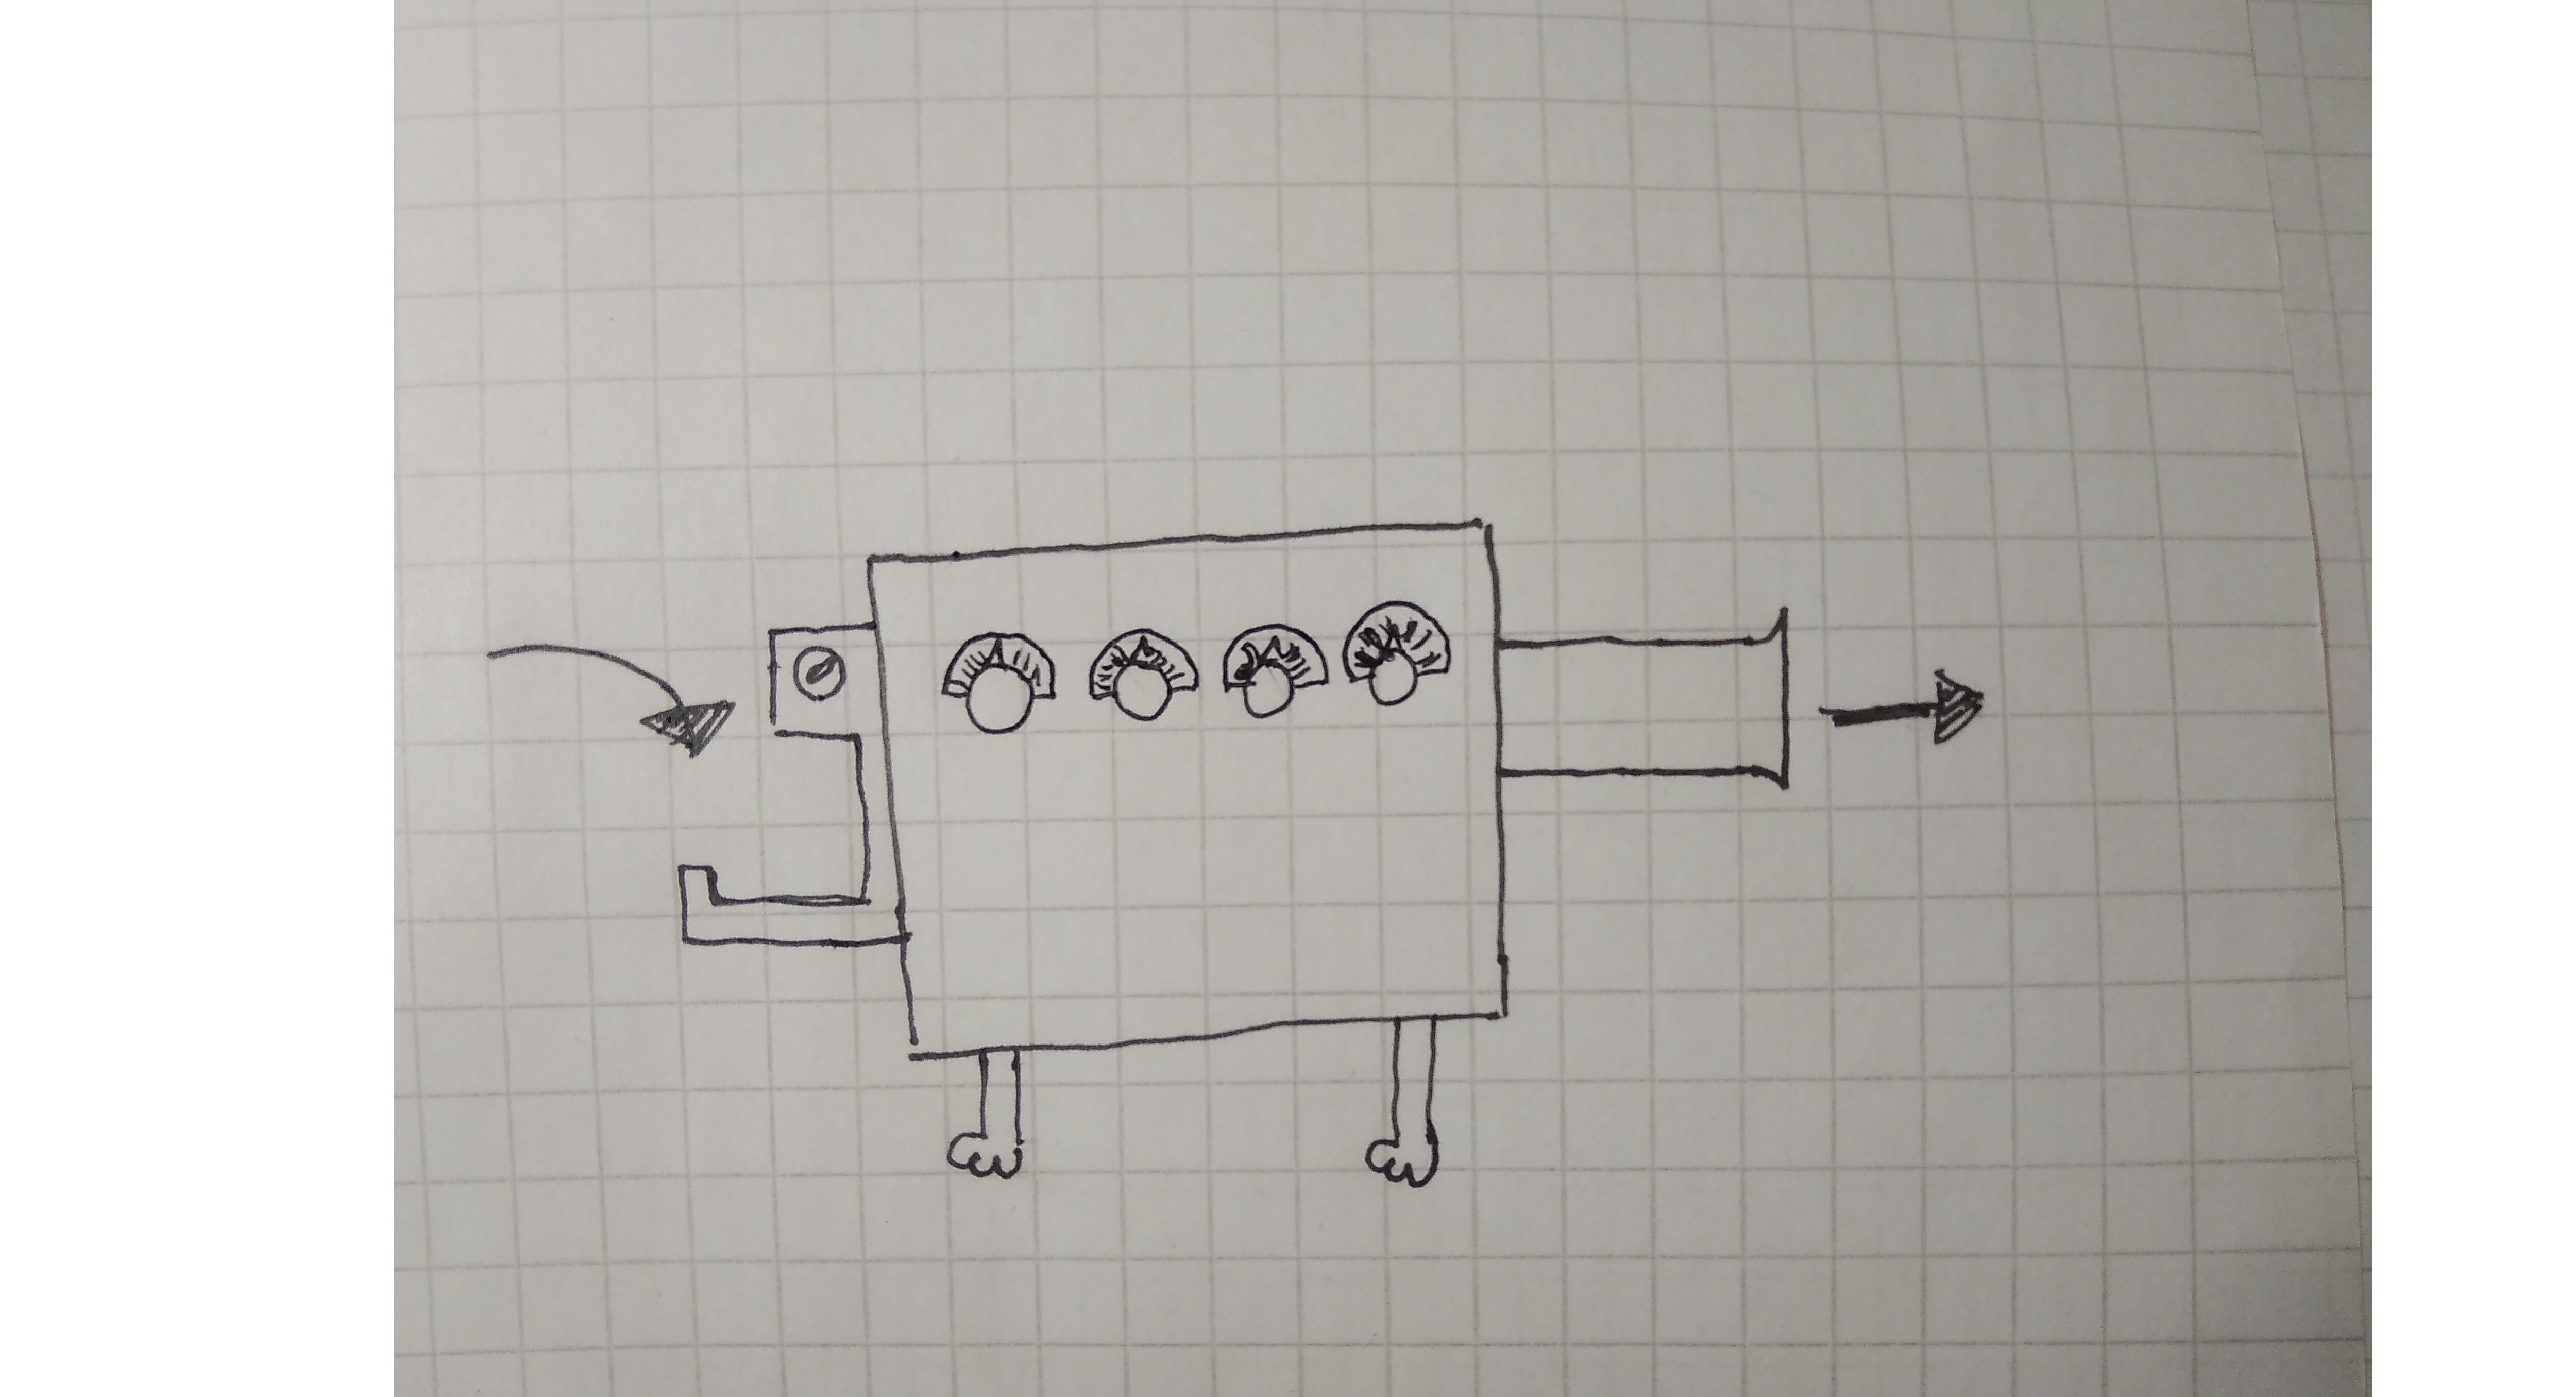
\includegraphics[width=0.9\textwidth]{malli_uusi.jpg}

% malli ja parametrit


\end{frame}

\begin{frame}{Mallit ovat yleisiä}

\includegraphics[width=0.9\textwidth]{mallit_ovat_yleisiä.jpg}


% malli on yleiskäyttöinen: Lasse ja MNIST ovat kysymysmerkki

\end{frame}

\begin{frame}{Mitä tarkoittaa parametrien oppiminen: optimointialgoritmi}

%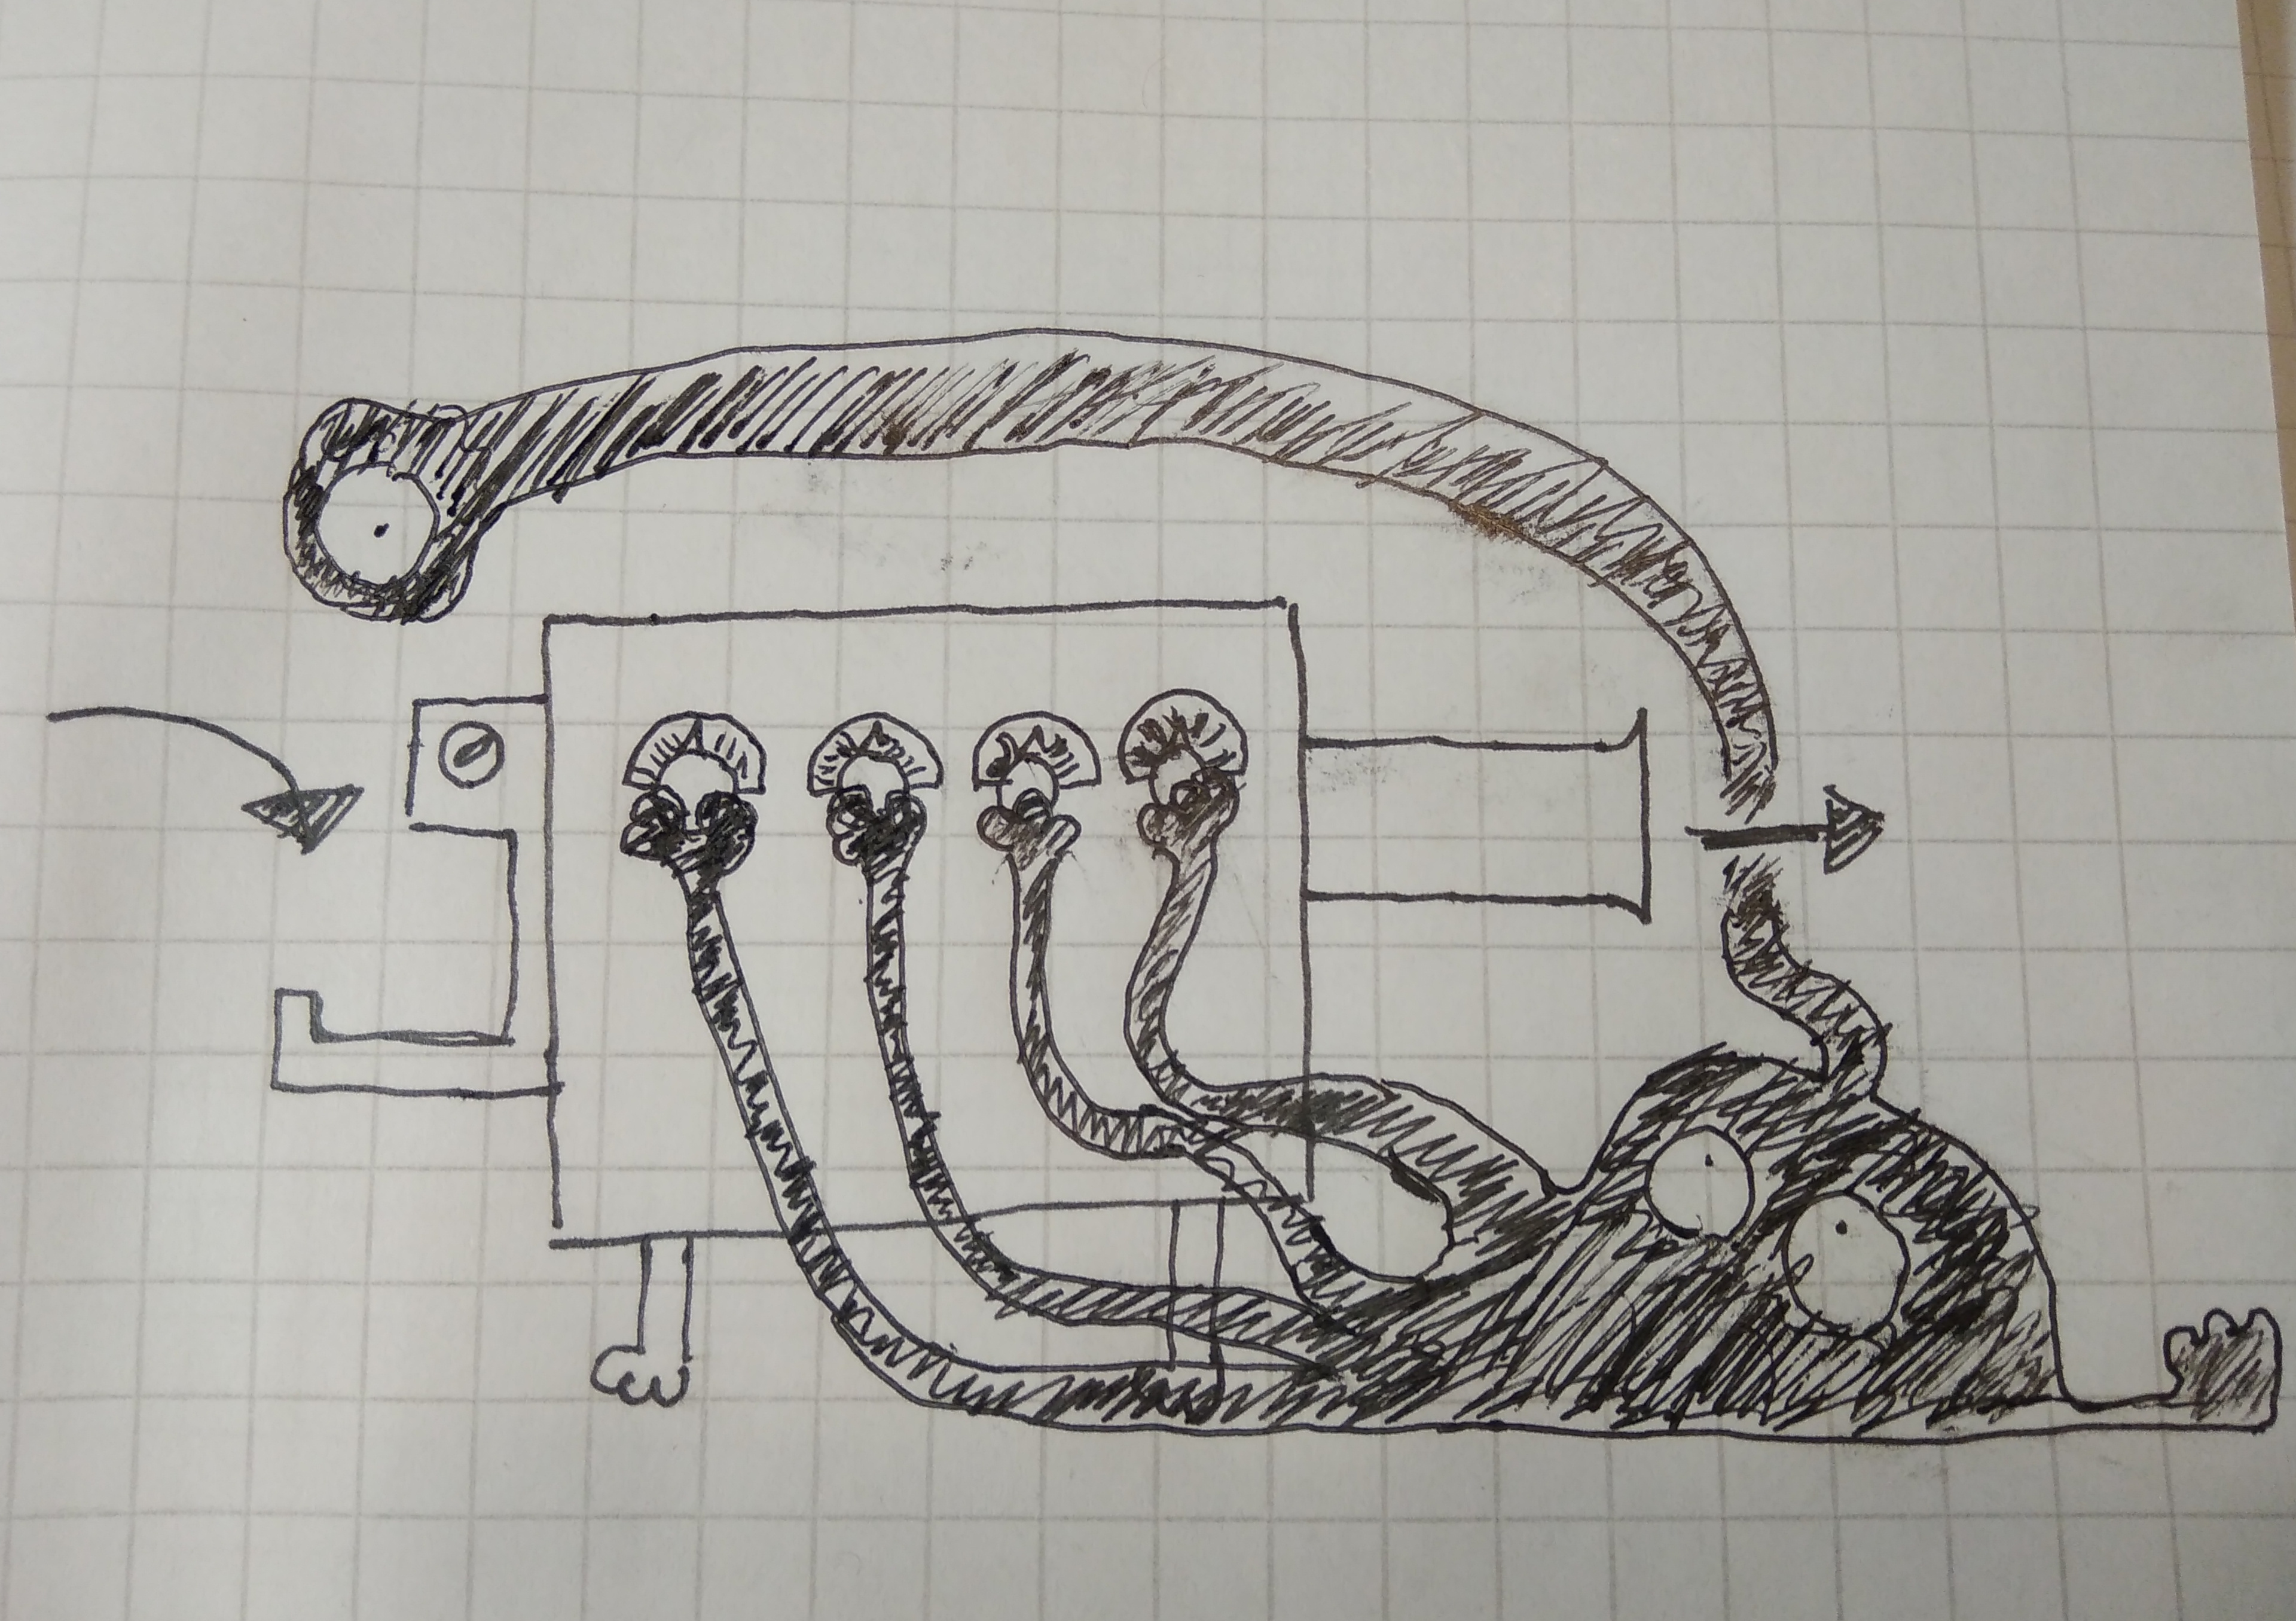
\includegraphics[width=0.7\textwidth]{malli_ja_parametrien_oppiminen.jpg}

% Mustekala säätää parametrit niin että Lasse on laiskiainen
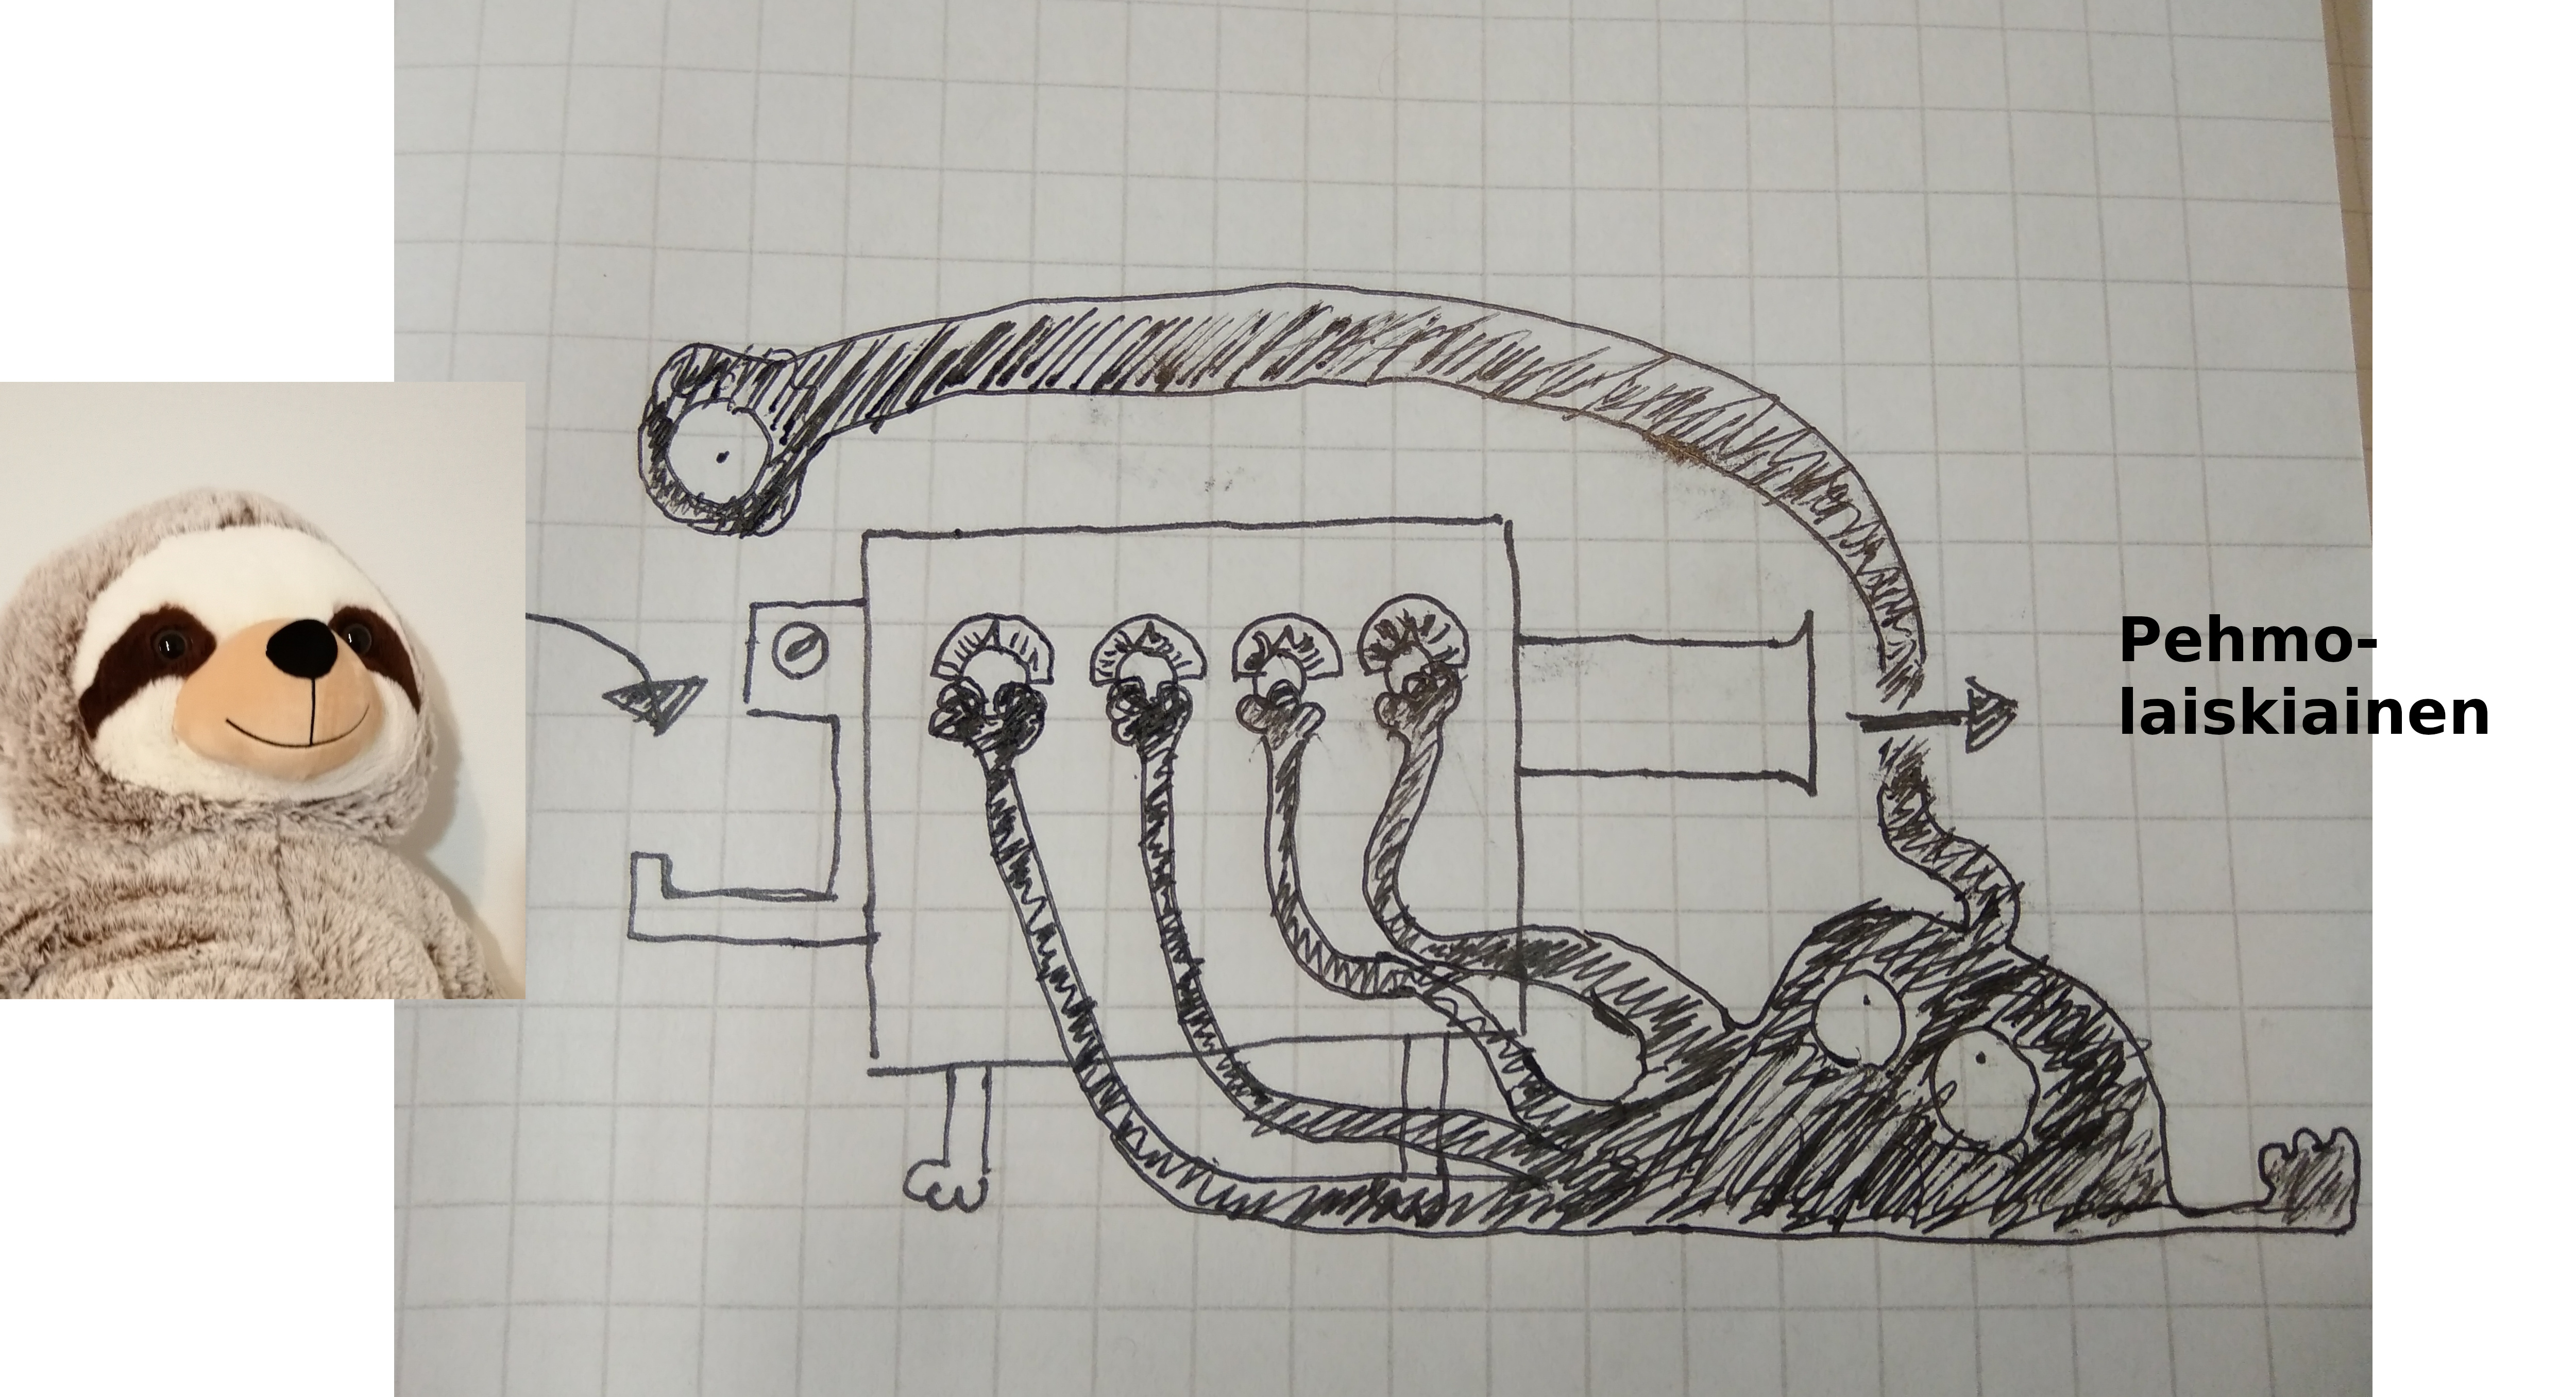
\includegraphics[width=0.9\textwidth]{malli_parametrit_lasse.jpg}


\end{frame}

\begin{frame}{Mitä tarkoittaa "tilastollisesti keskimäärin oikea vastaus"?}

Tähän on tarkka matemaattinen vastaus$\to$ ei sillä väliä.

\pause
\begin{block}{Eräs käytännöllinen esimerkki:}

\begin{enumerate}
    \item<2-> Valitaan sääntö jolla mitata virheellisen vastauksen virheellisyyttä numerolla.
    \item<3-> Jätetään sivuun osa datasta jota ei käytetty oppimiseen. (Testijoukko.)
    \item<4-> Mitataan opetetun koneen vastausten virhe testijoukossa.
\end{enumerate}

\end{block}


\end{frame}

\begin{frame}{\textbf{Tilastollisesti} keskimäärin oikea vastaus: Ristiinvalidointi}

Pätkitään data palasiin monta kertaa ja mitataan virhe monta kertaa!

	\begin{figure}
				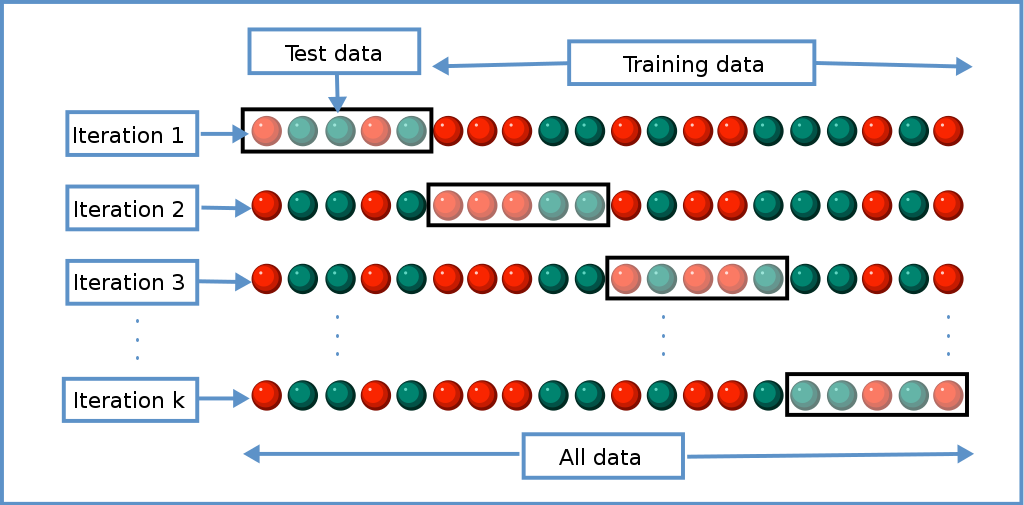
\includegraphics[width=\textwidth]{kfold_wikipedia.png} \
				\caption*{ Lähde: Wikipedia, User:Gufosowa, CC BY-SA 4.0 [2]}
	\end{figure}

%https://en.wikipedia.org/wiki/File:K-fold_cross_validation_EN.svg
    
\end{frame}

\begin{frame}{Tiivistelmä johdannosta:}
    Tilastollisesti oppiva kone:
    \pause
    \begin{enumerate}
        \item Algoritmi joka ei opi (esimerkki quicksort): olemme kirjoittaneet sen niin että se antaa taatusti oikeita vastauksia.
        \item Algoritmi joka oppii (esimerkiksi tämä esitelmä:) emme osaa / jaksa kirjoittaa algoritmia joka antaisi taatusti oikeita vastauksia.
        Sen sijaan valitsemme yleisen mallin, jonka parametrit voimme säätää (opettaa) niin että se antaa keskimäärin oikeita vastauksia
        \item Keskimäärin oikean vastauksen arviointi:
    \end{enumerate}
    
\end{frame}


\section{Ensimmäinen eläin: Logistinen regressio}

\begin{frame}{}
  \tableofcontents[currentsection]
\end{frame}

\begin{frame}{Eläinosion idea}
    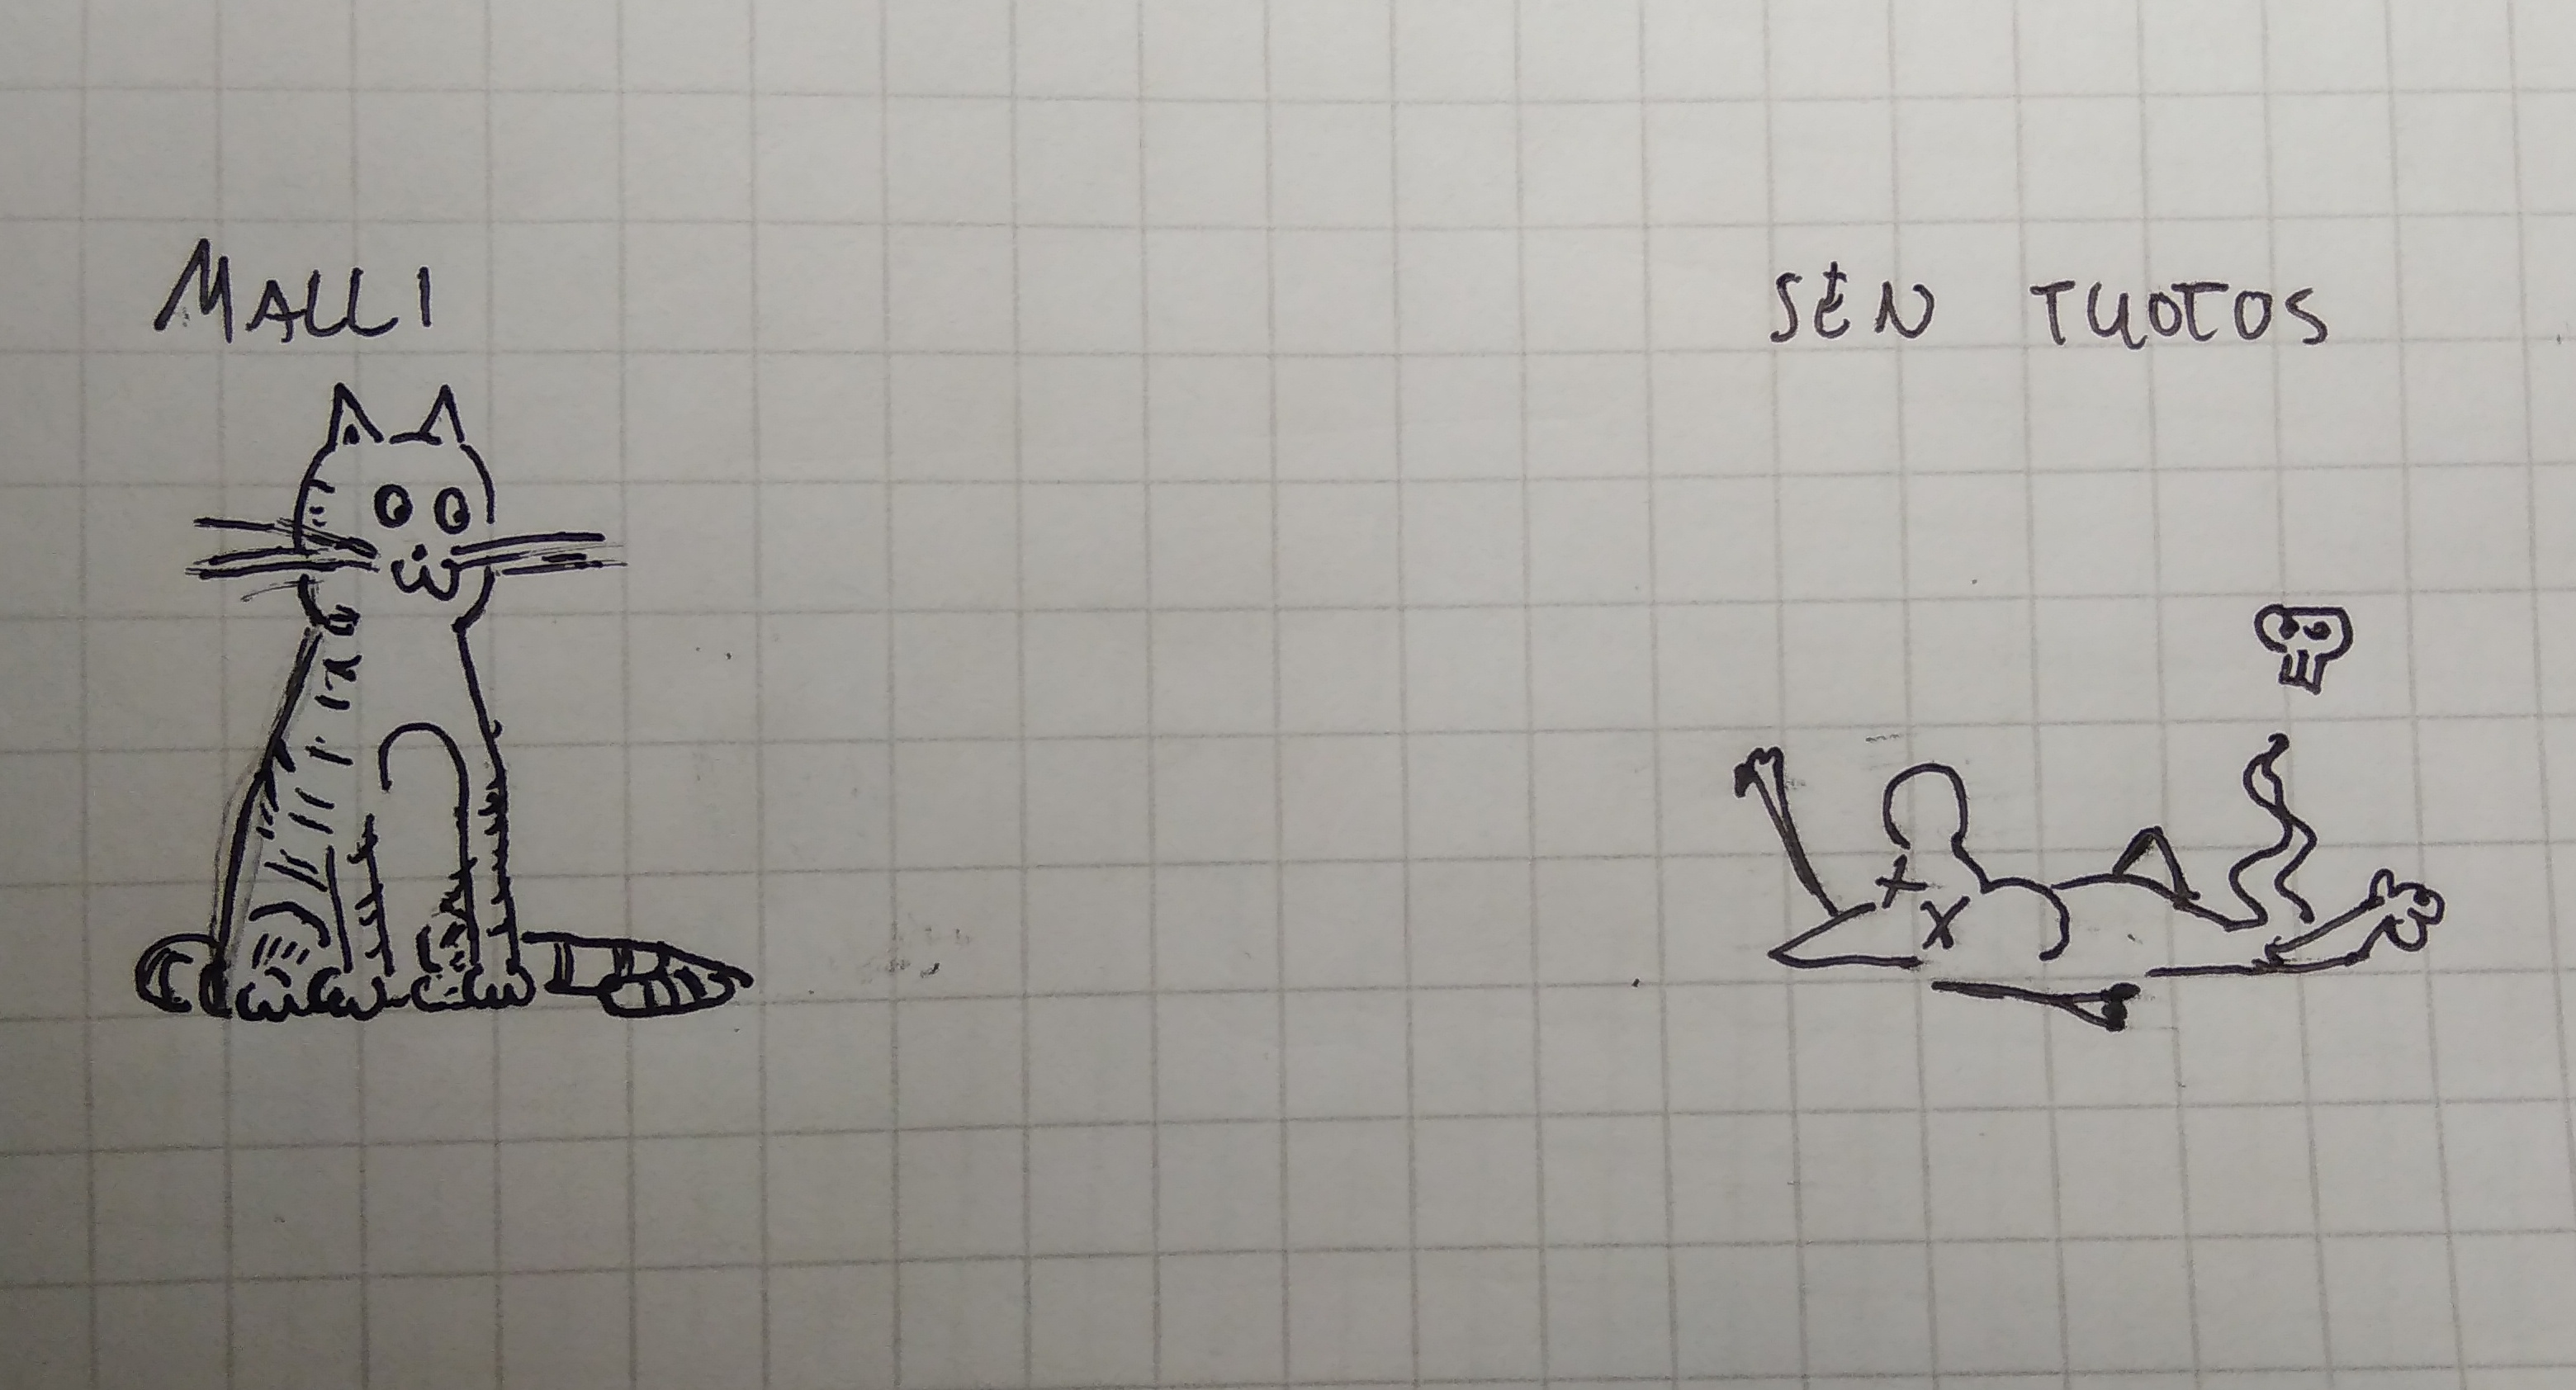
\includegraphics[width=0.9\textwidth]{malli_tuotos.jpg}
\end{frame}

\begin{frame}{Mistä eläinosiossa ei puhuta}
        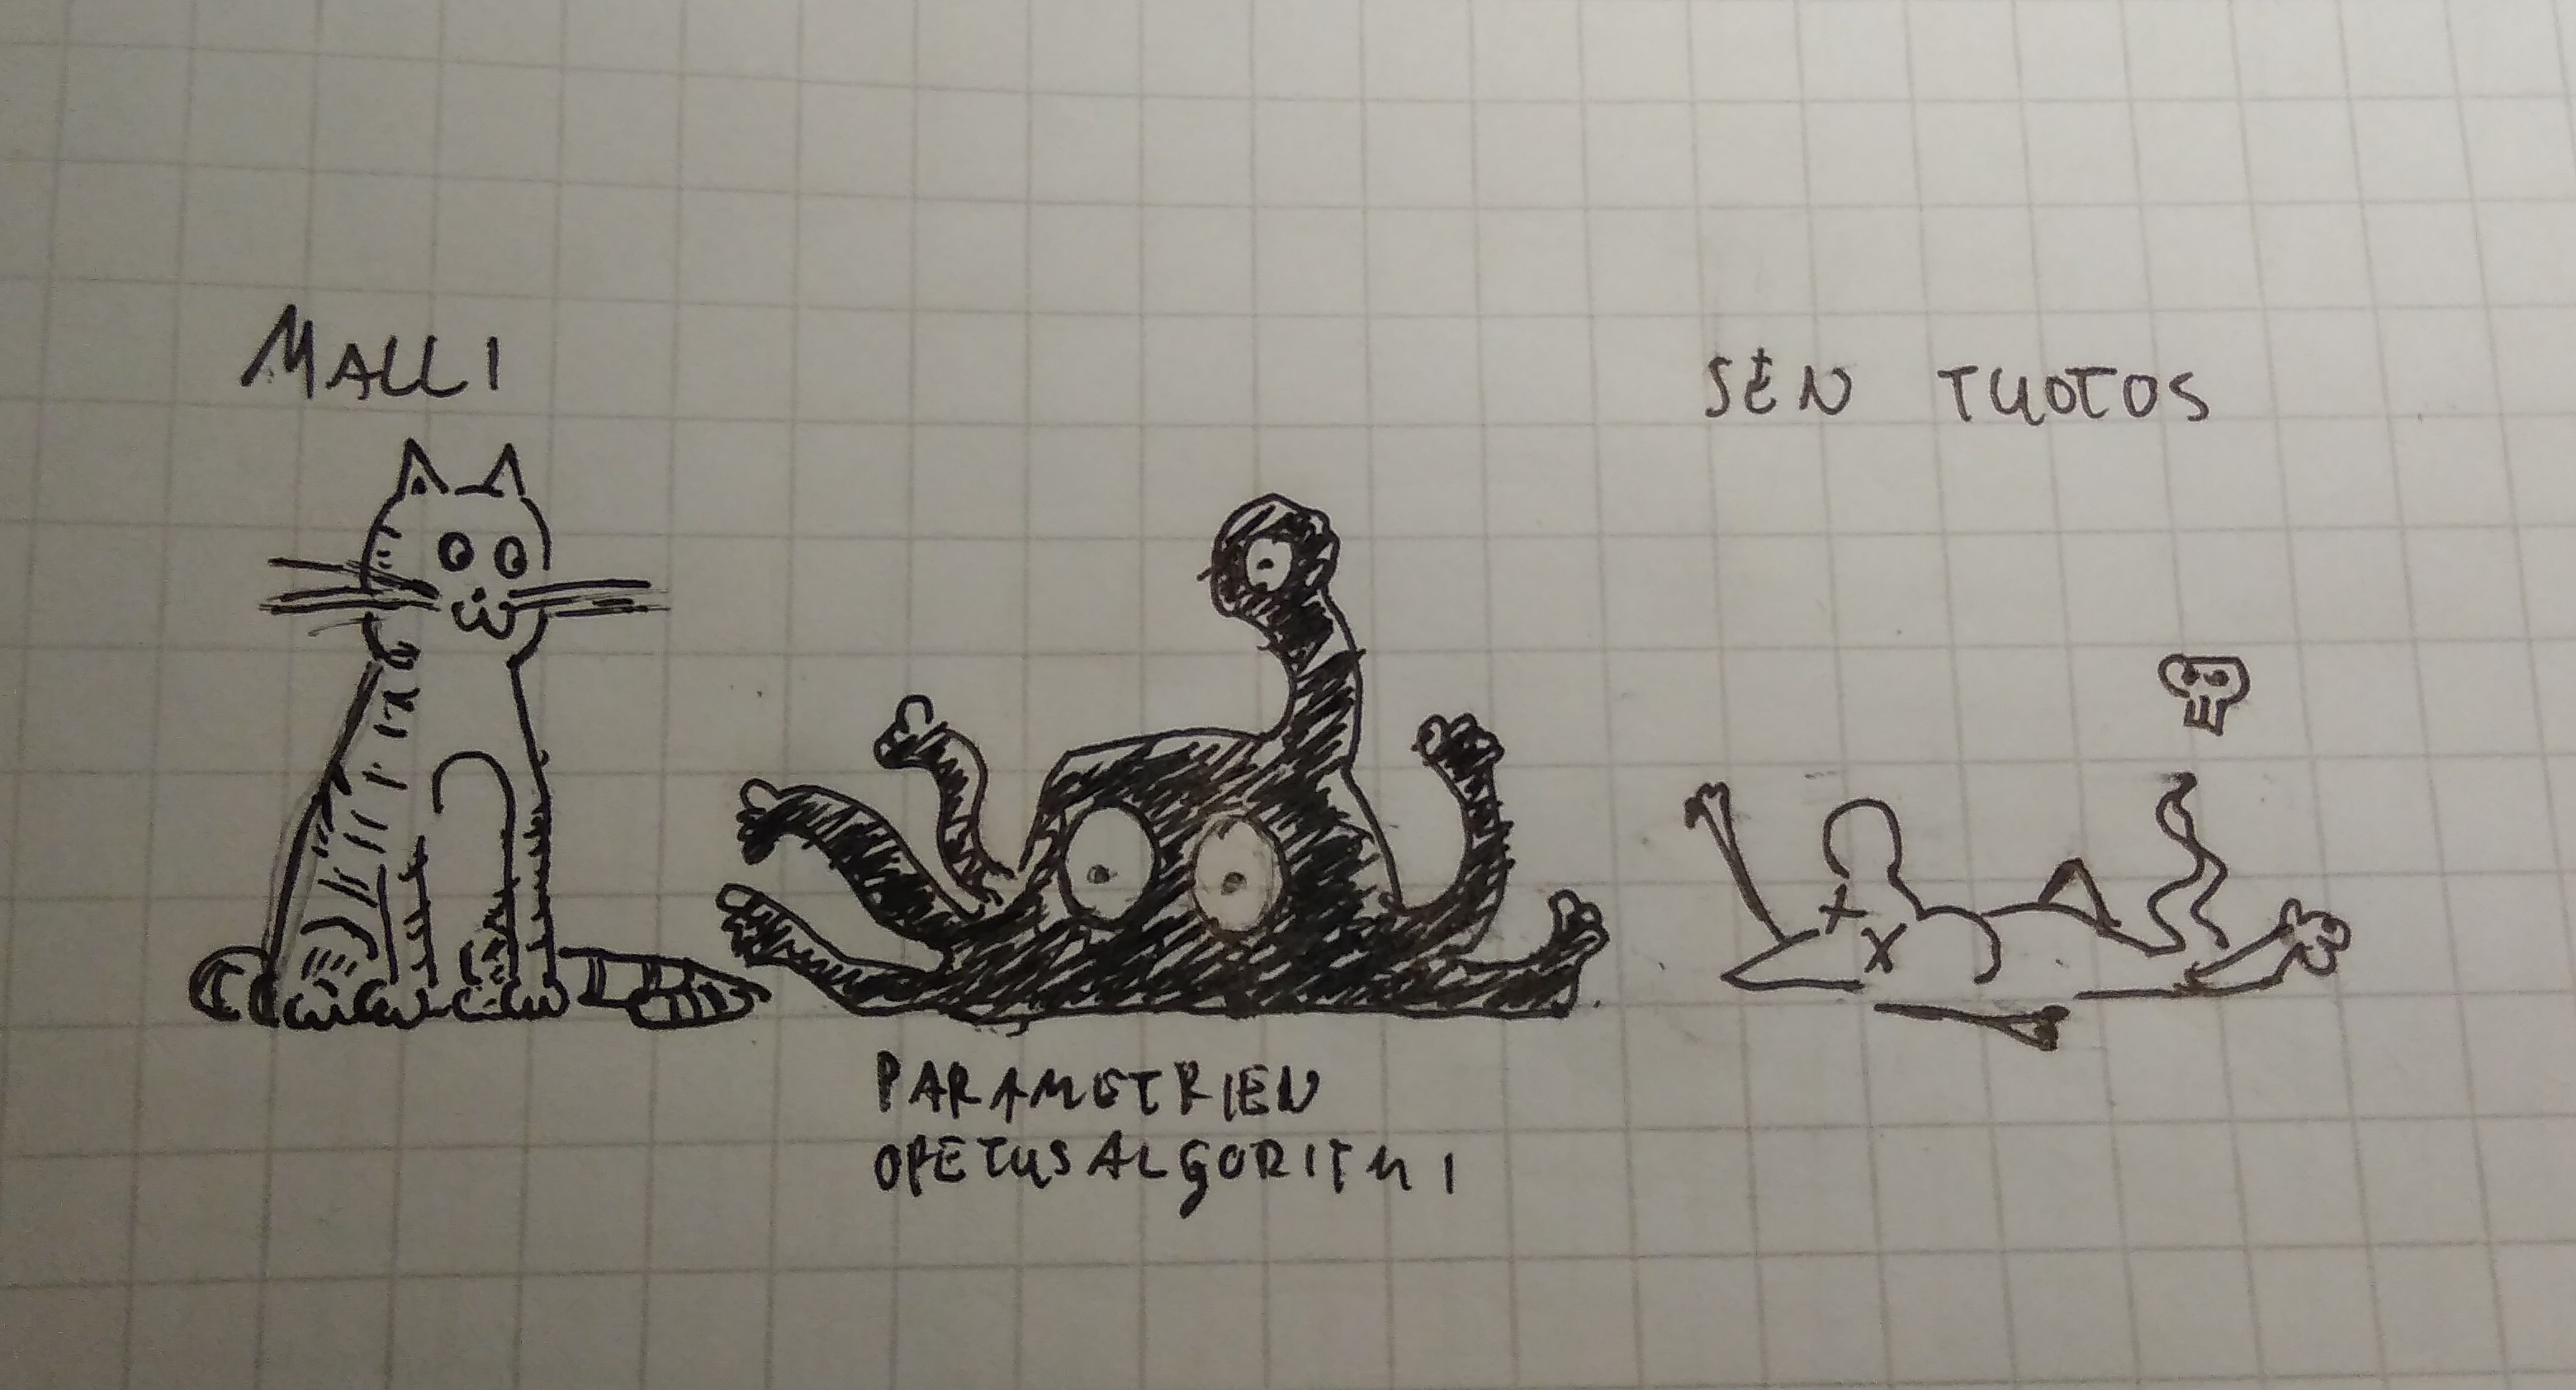
\includegraphics[width=0.9\textwidth]{malli_tuotos_optimointi.jpg}

\end{frame}

\begin{frame}{Eläinosion esimerkkidata: MNIST}
    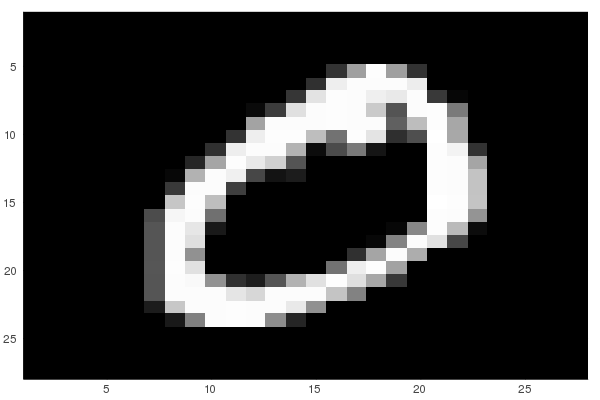
\includegraphics[width=0.4\textwidth]{mnist2.png}
    
    60000 käsinkirjoitettua numeroa jotka käsitelty kivasti.
\end{frame}

\begin{frame}{Logistinen regressio: Visuaalinen johdanto}
    
\end{frame}

\begin{frame}{Lineaarinen regressio yhdellä kuvalla}
        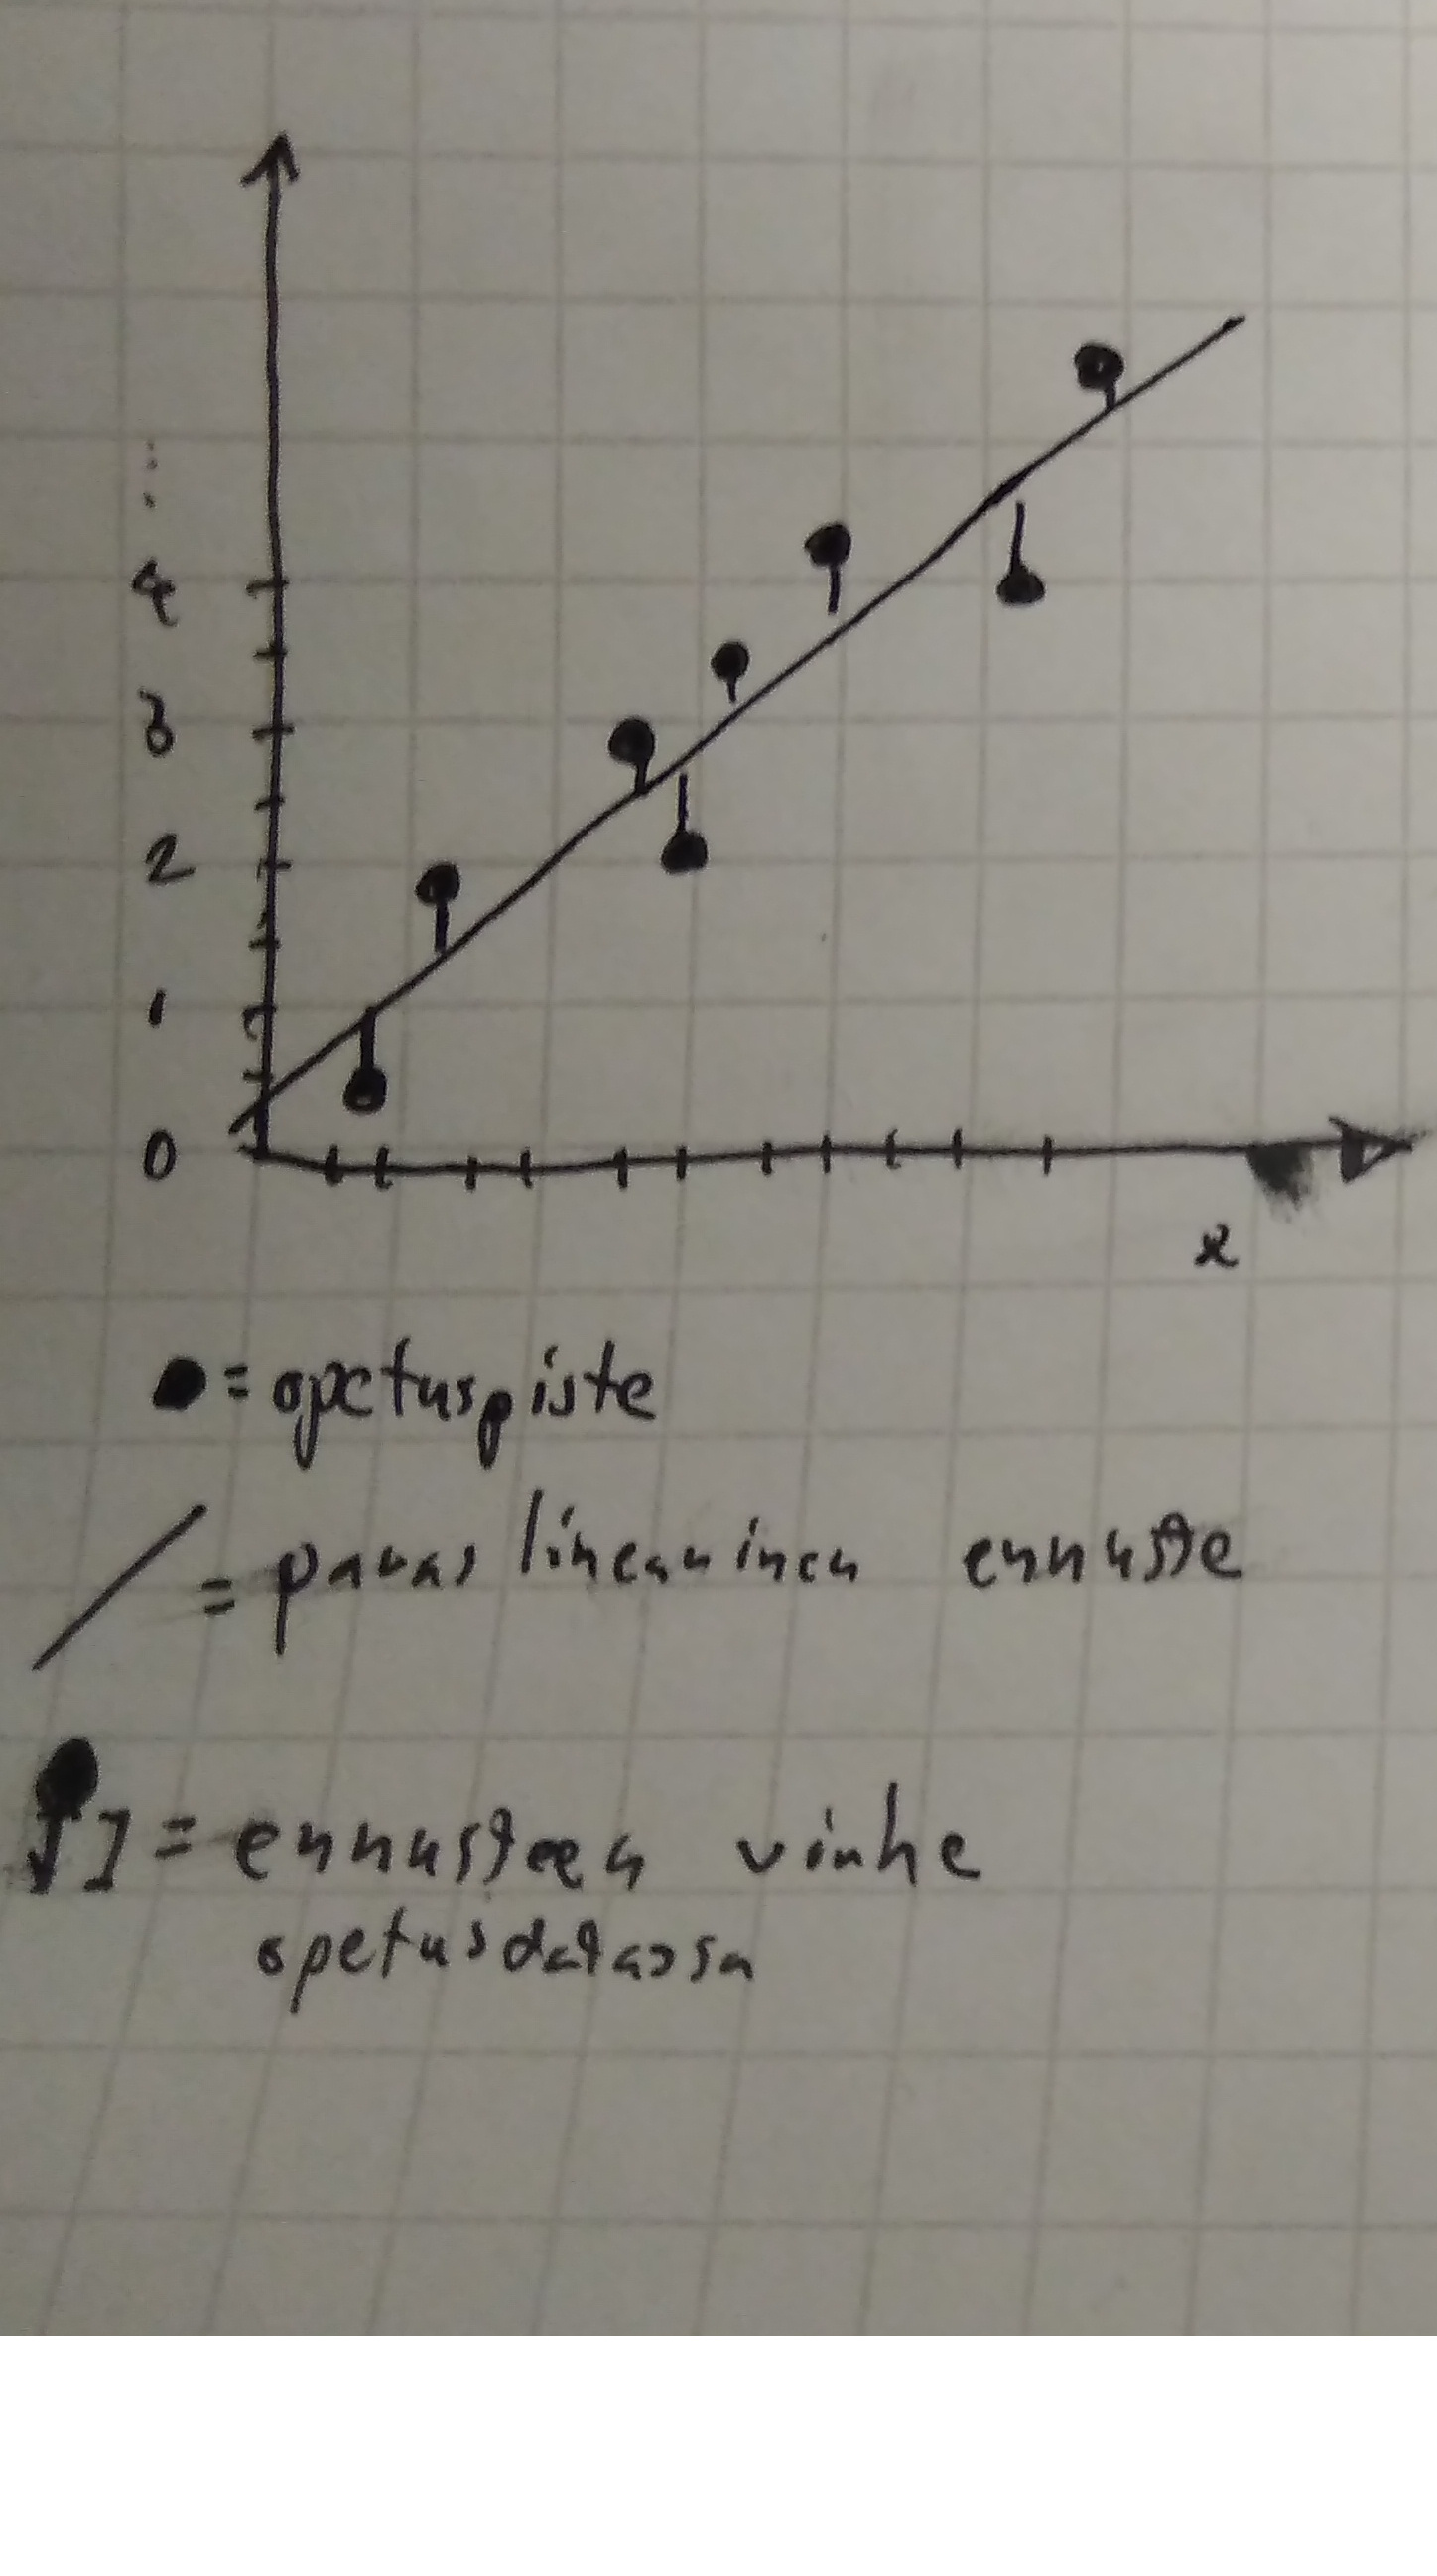
\includegraphics[width=0.4\textwidth]{lineaarinen1.jpg}
\end{frame}

\begin{frame}{Logistinen regressio kahdella kuvalla: 1}
    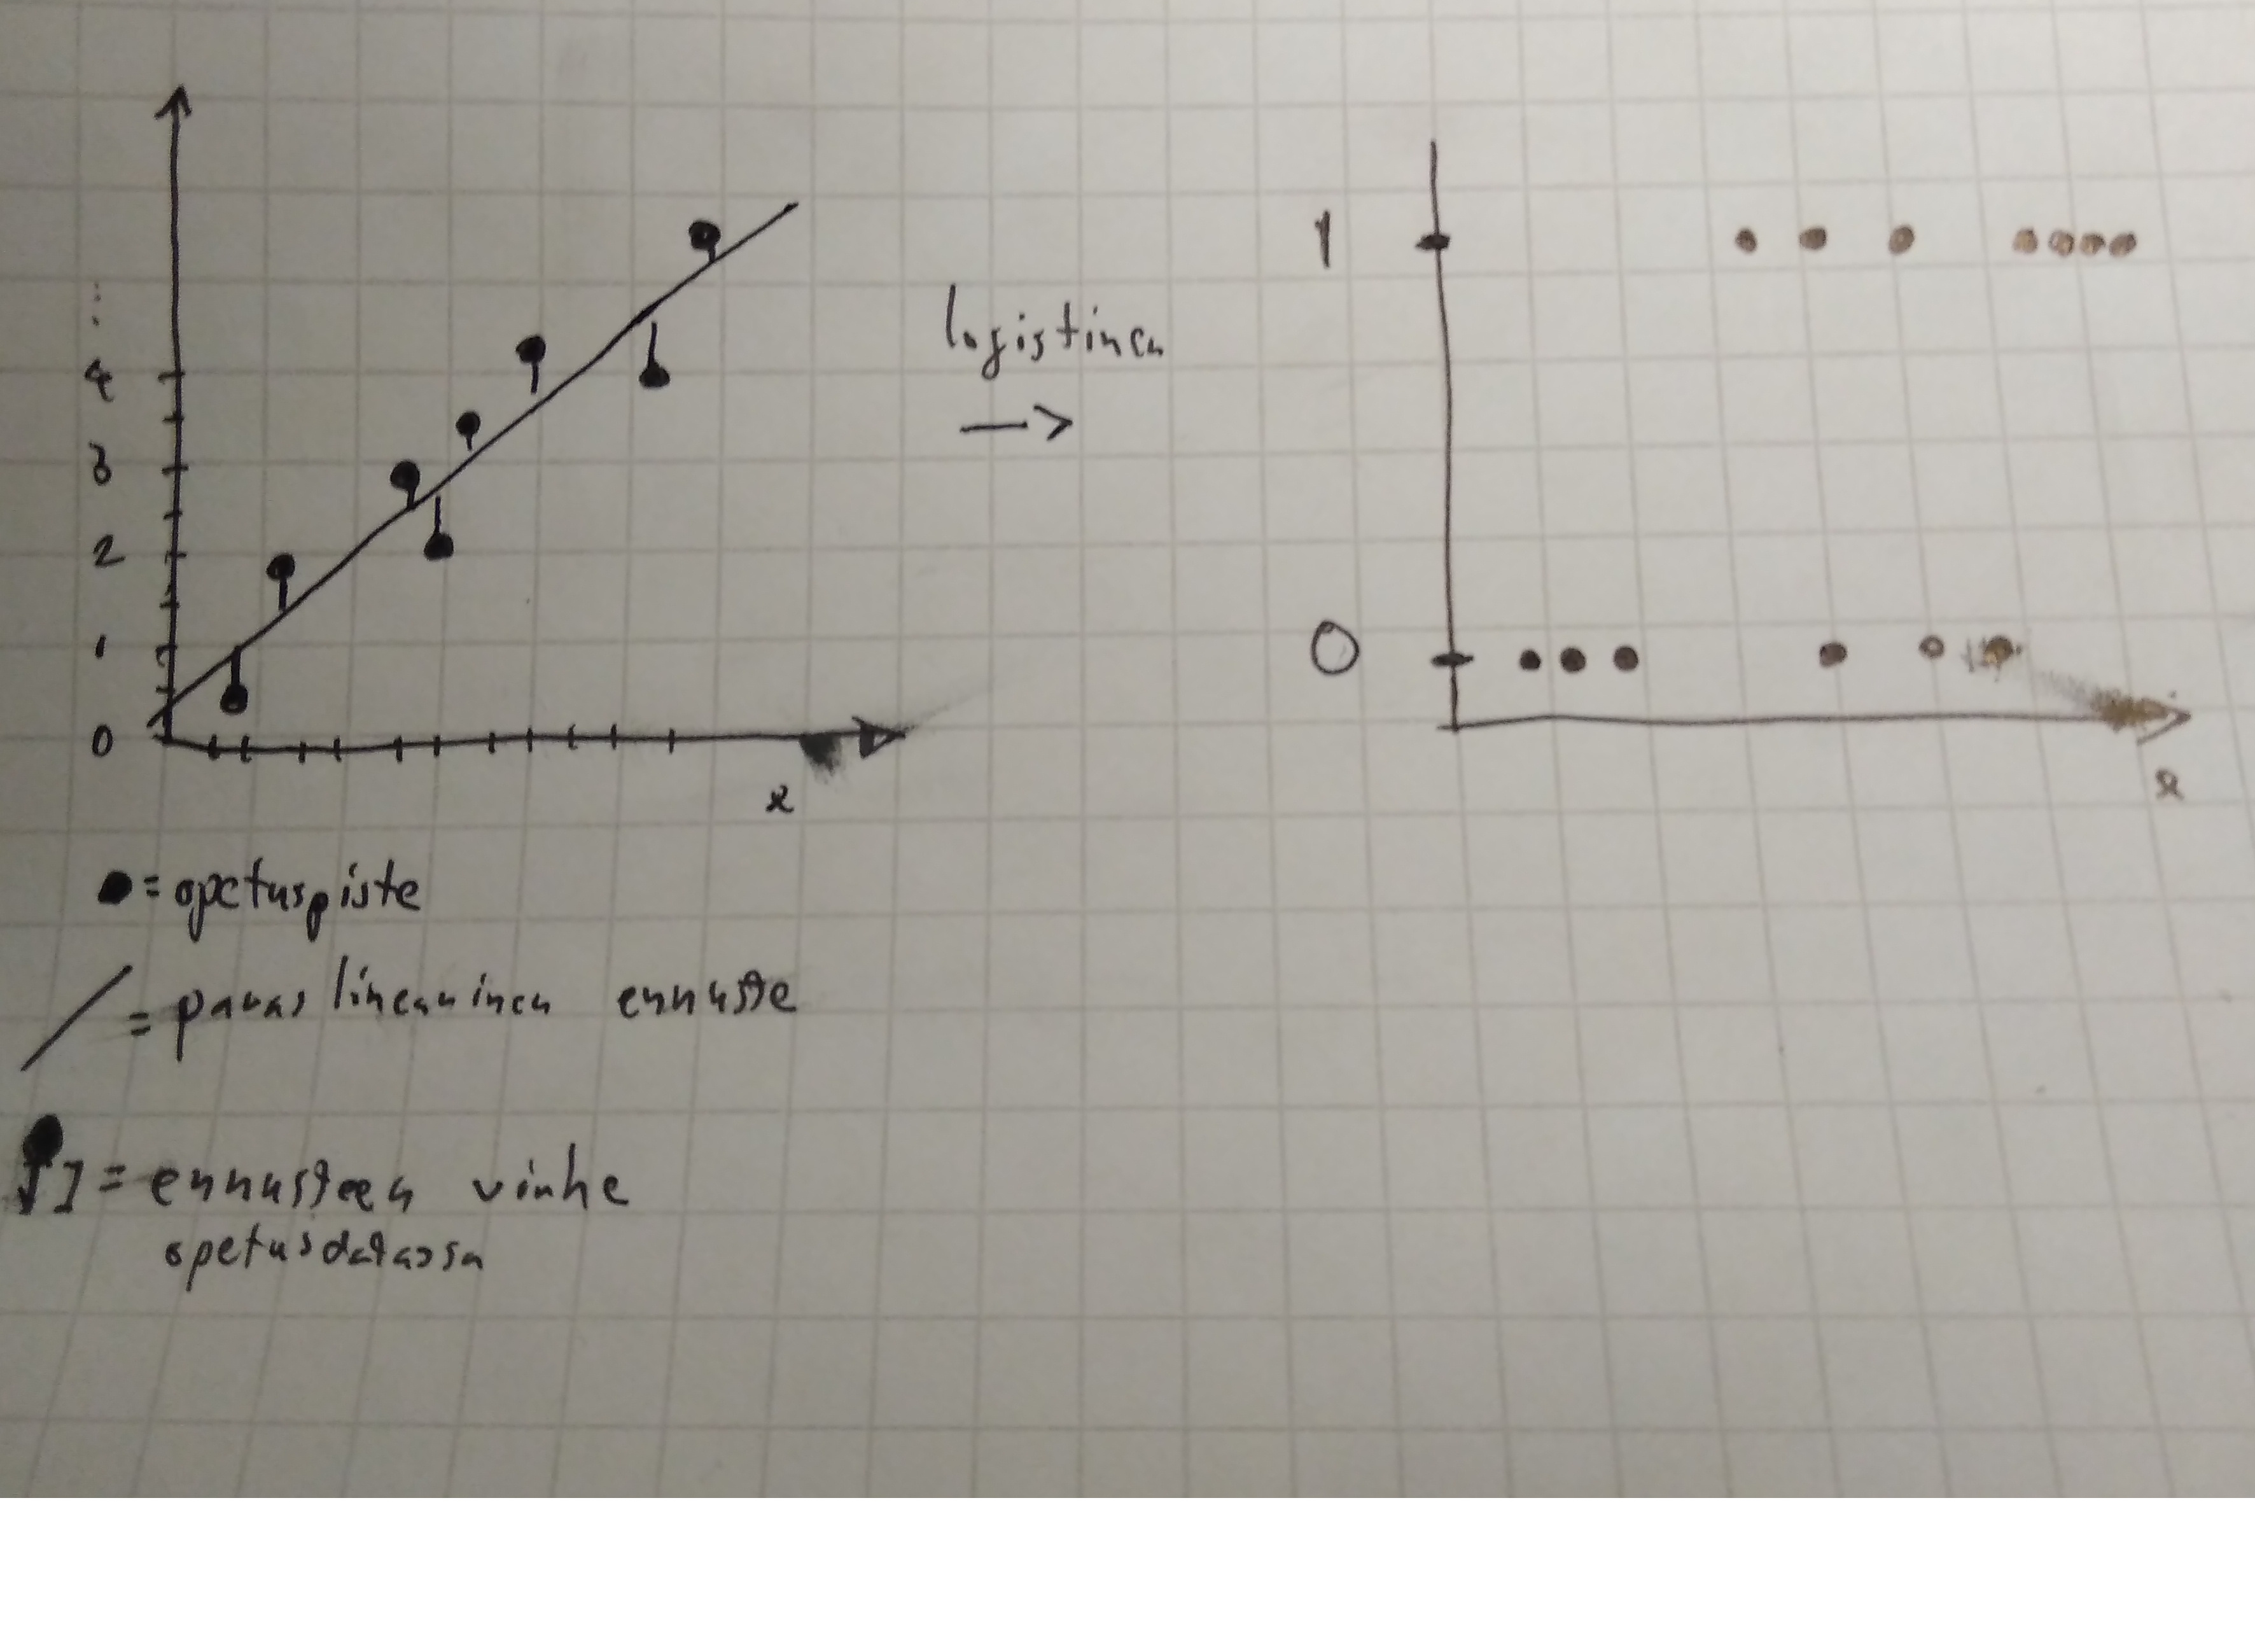
\includegraphics[width=0.8\textwidth]{logistinen1.jpg}
\end{frame}

\begin{frame}{Logistinen regressio kahdella kuvalla: 2}
    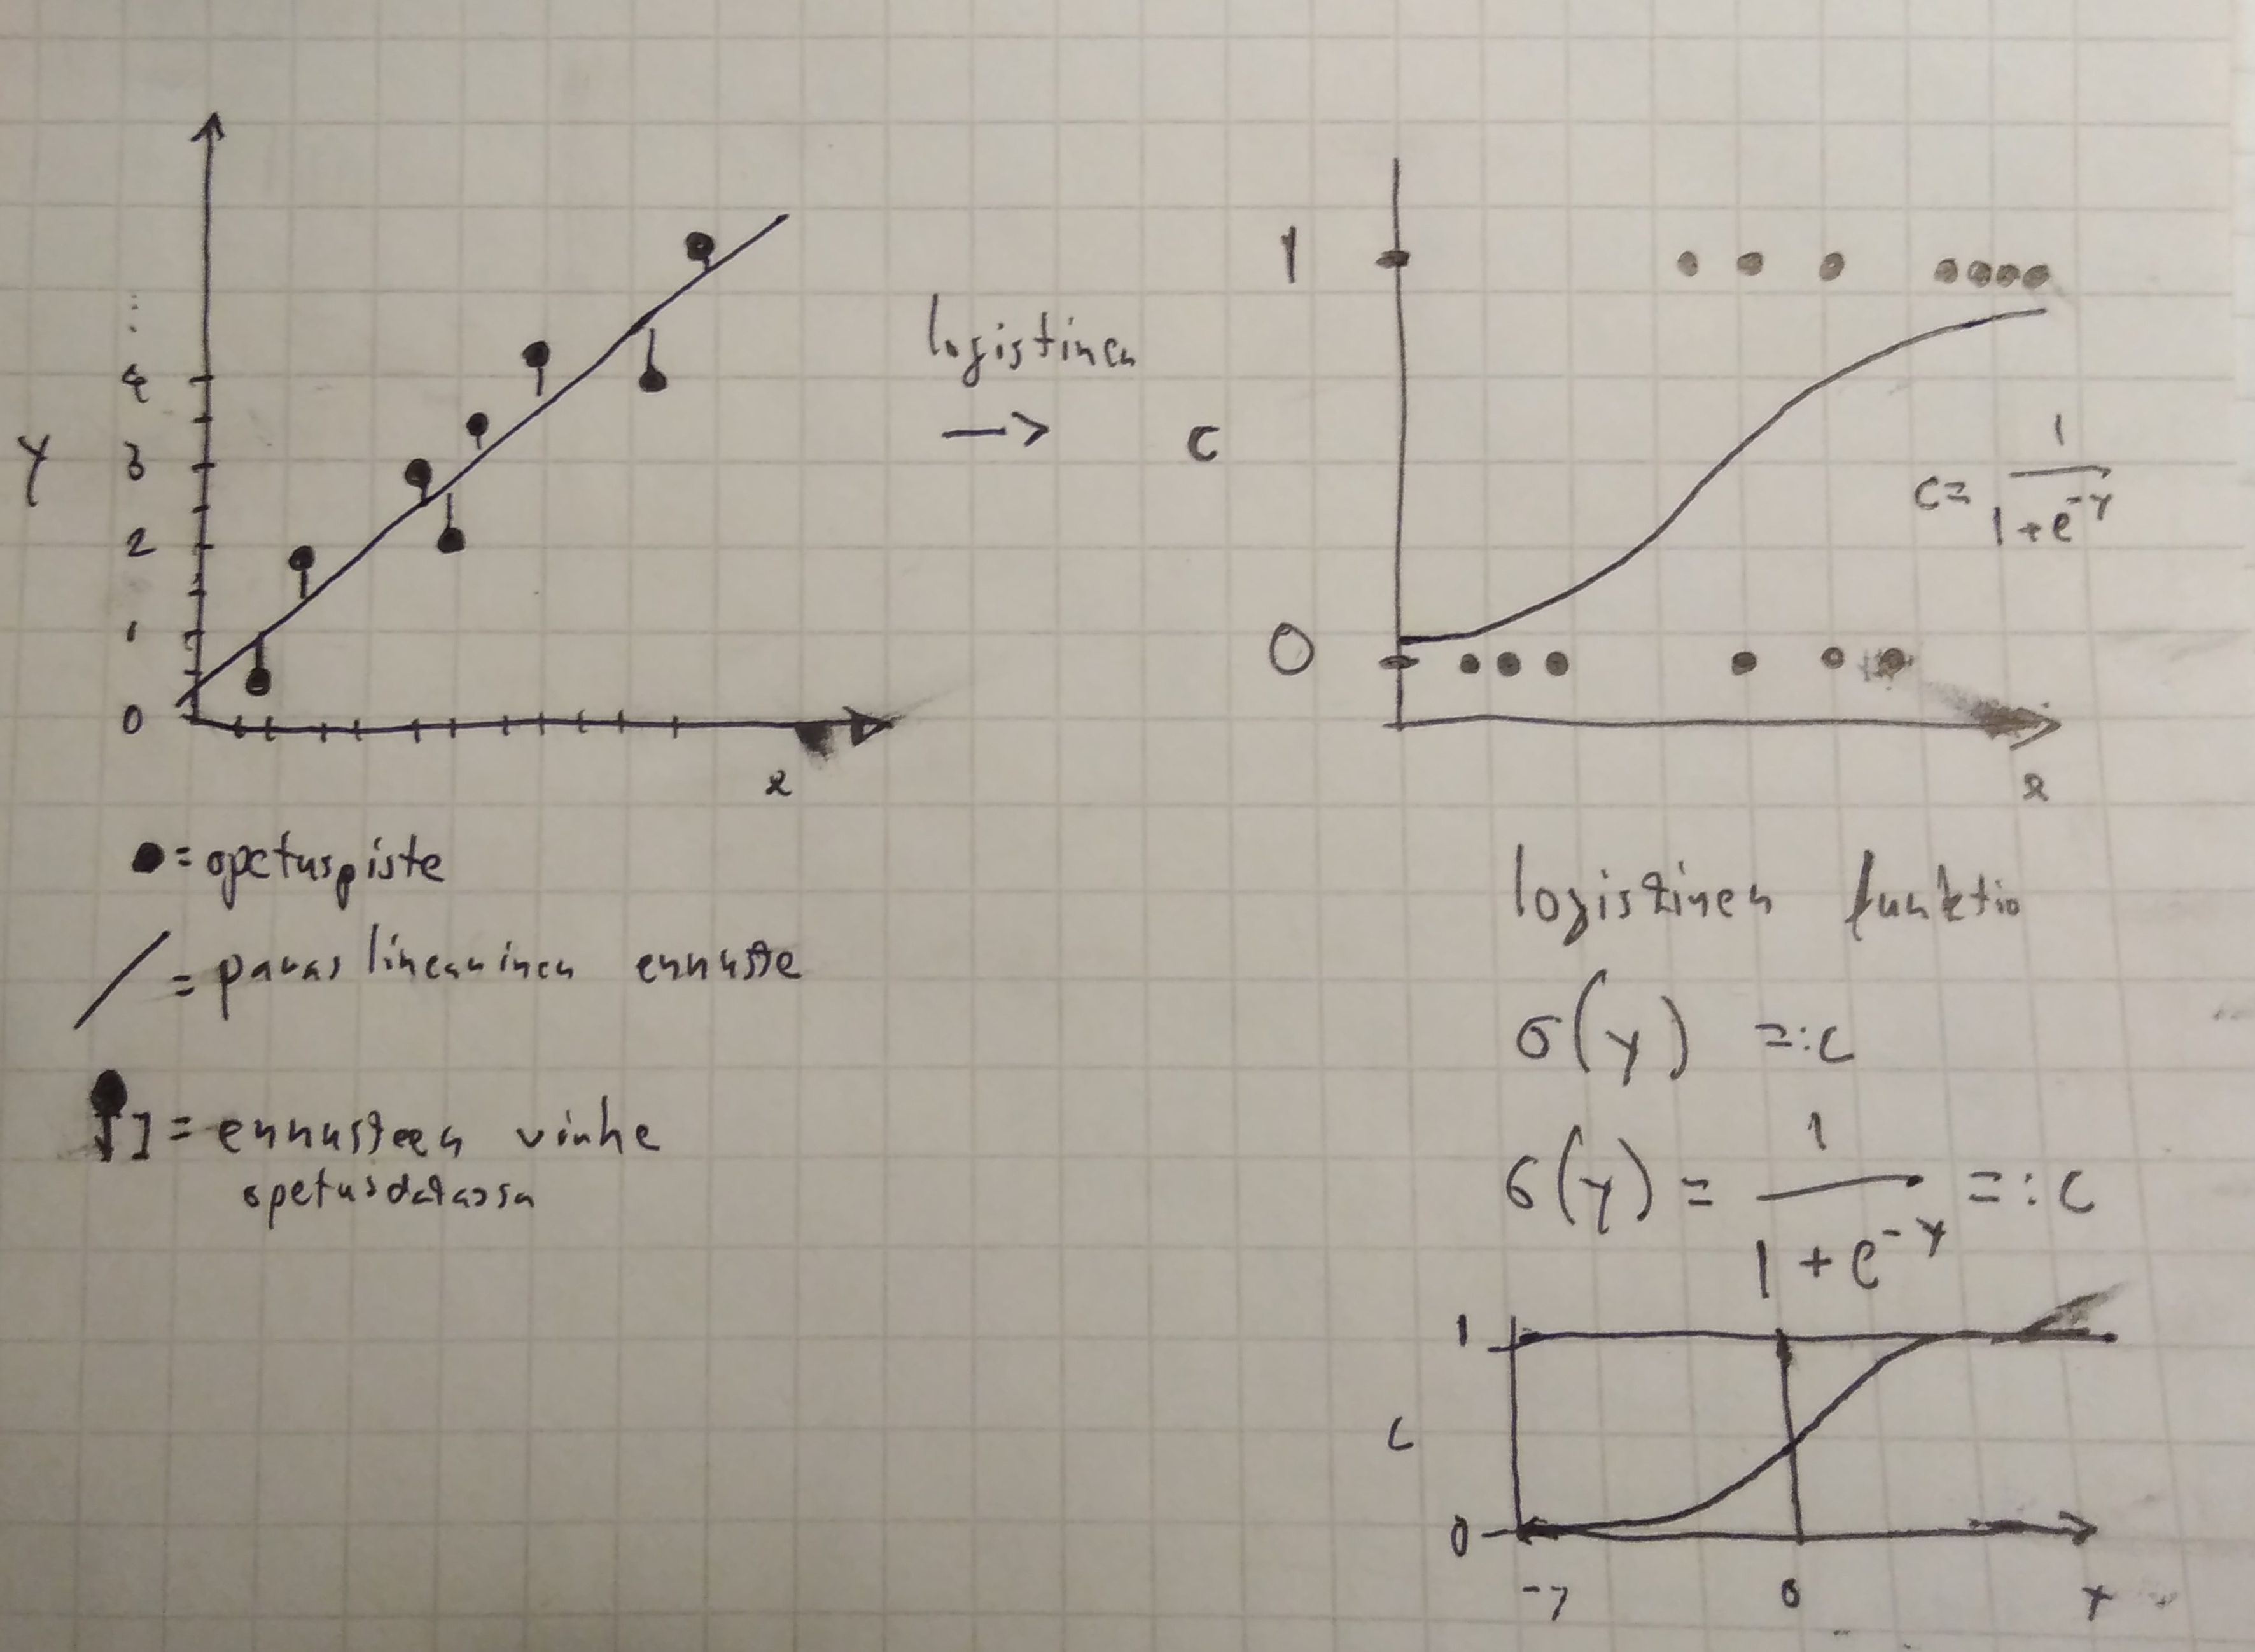
\includegraphics[width=0.8\textwidth]{logistinen2.jpg}
\end{frame}

\begin{frame}{Huijasin: Kolmas kuva}
    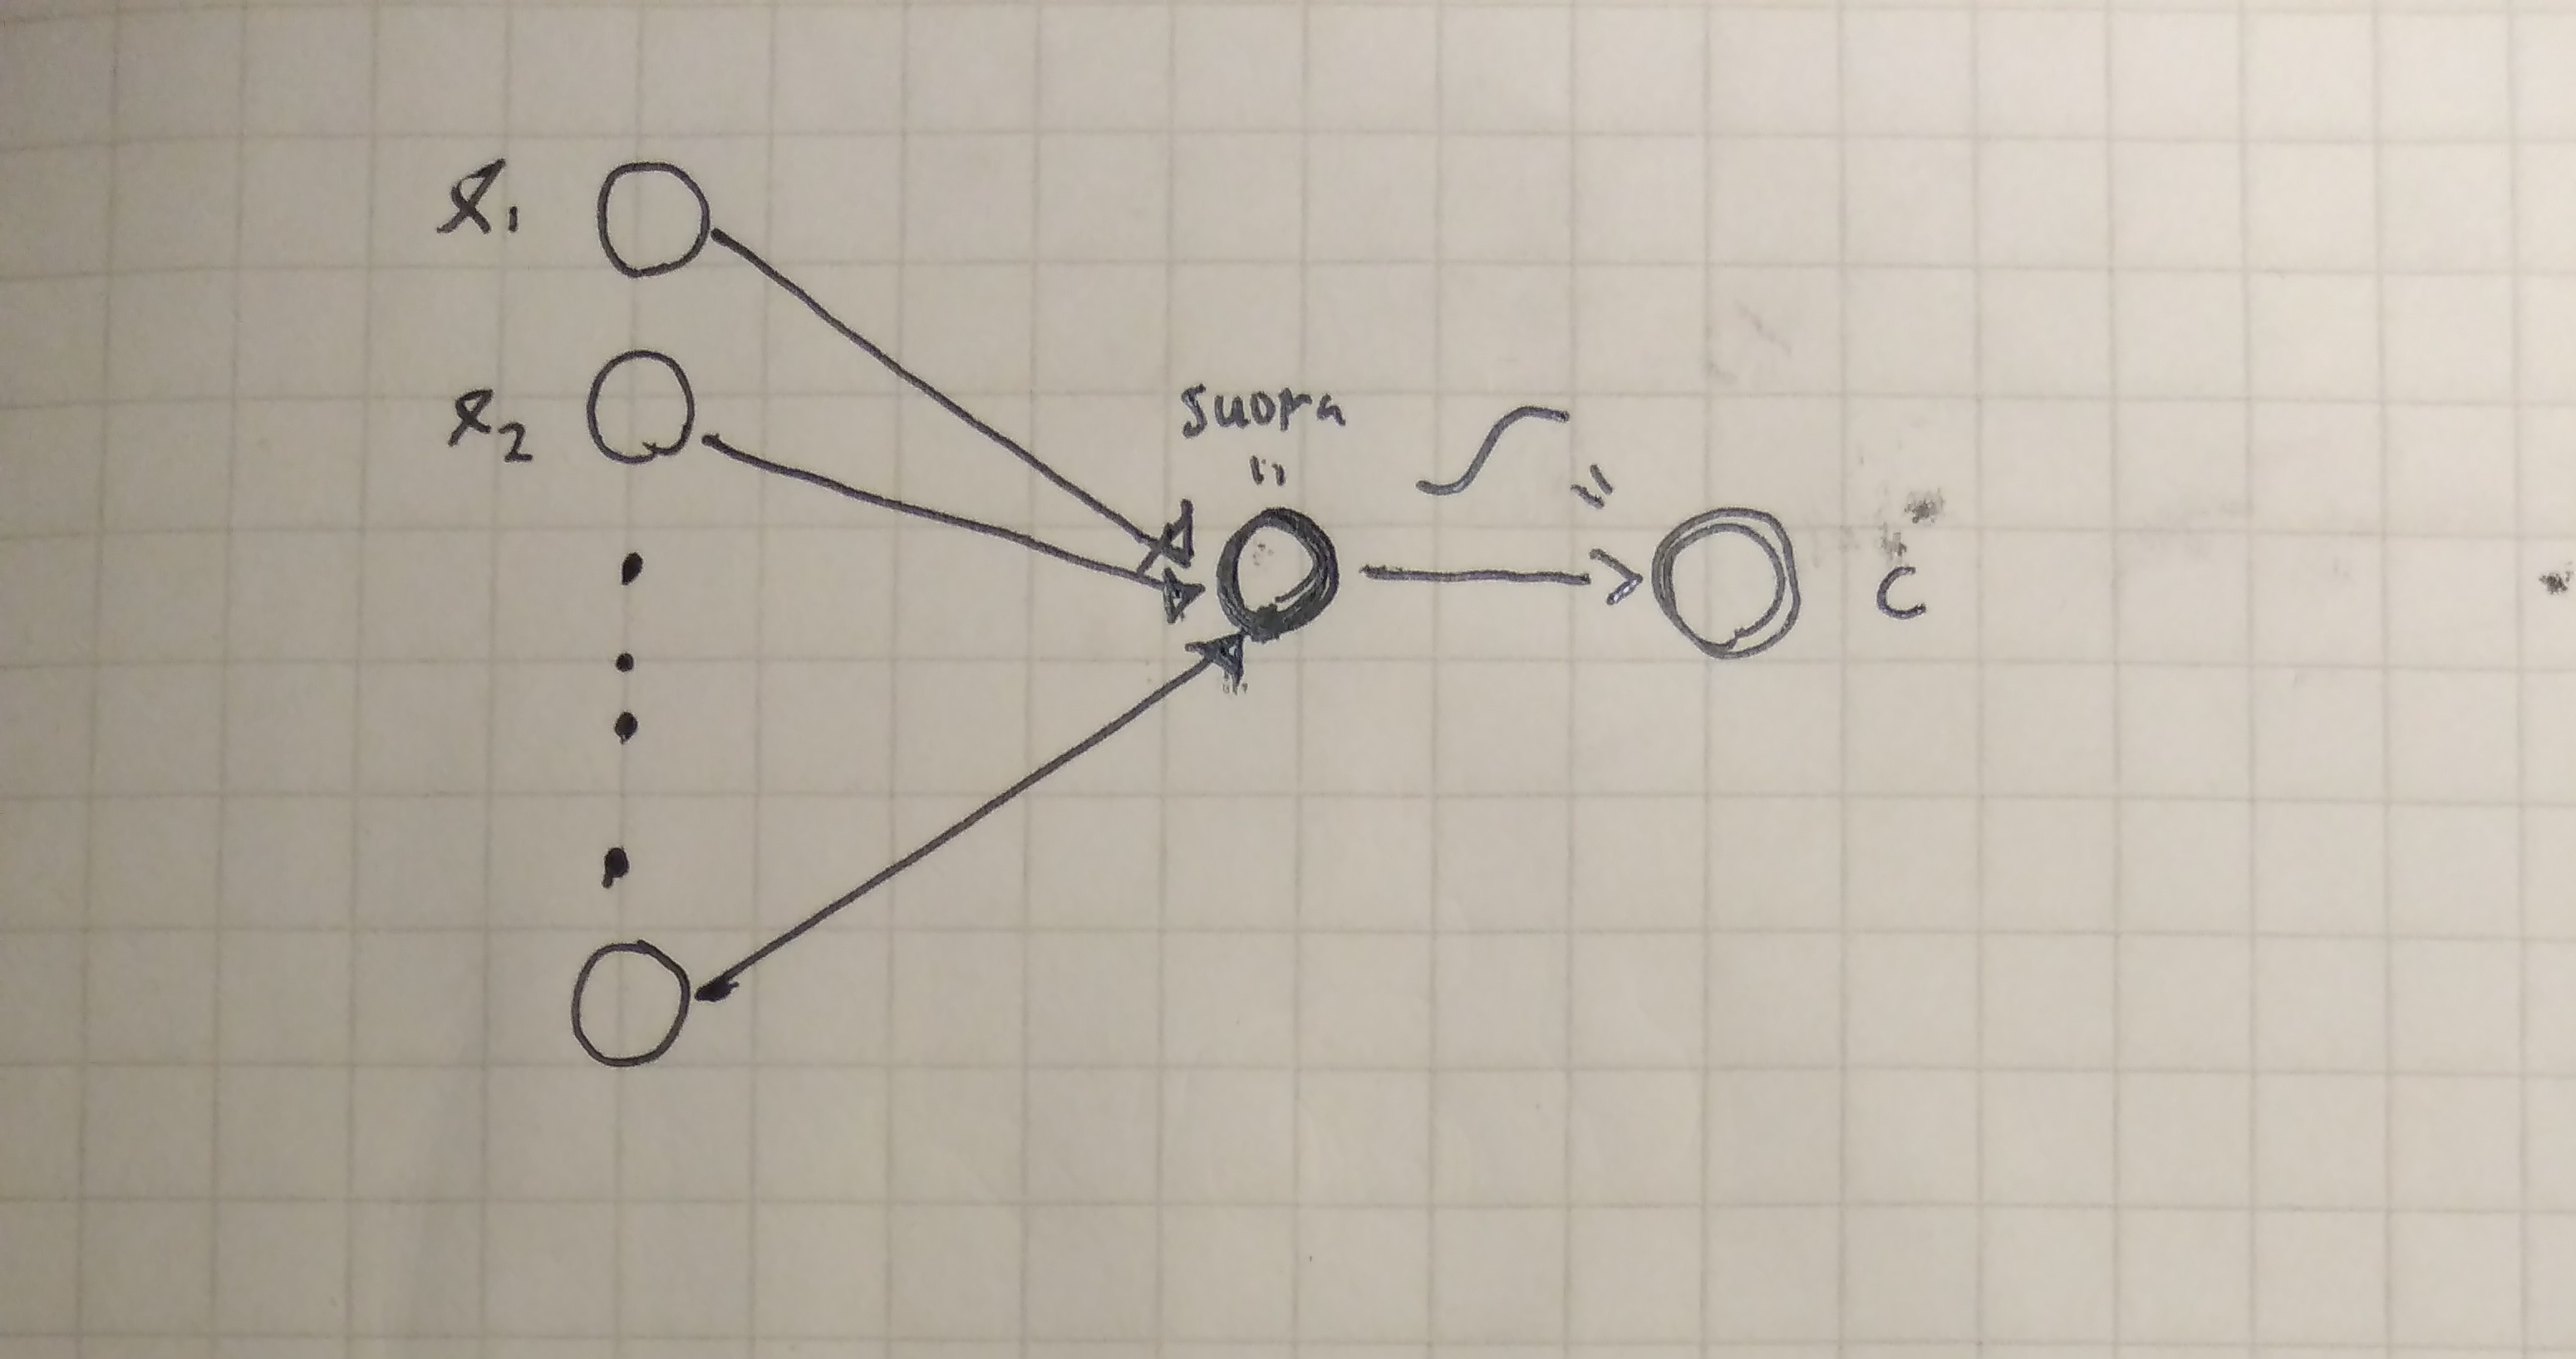
\includegraphics[width=0.8\textwidth]{logistinen_perceptron.jpg}
\end{frame}

\section{Toinen eläin: Yksinkertainen neuroverkko}

\begin{frame}{}
  \tableofcontents[currentsection]
\end{frame}

\begin{frame}{Neuroverkot \textbf{hyvin} ytimekkäästi}
    
\end{frame}

\begin{frame}{Pari sanaa neuroverkoista ja oikeista hermosoluista}
    \begin{itemize}
        \item<1-> Ihmisten, nisäkkäiden, muiden \textbf{hermoverkot}: yksittäiset hermosolut ovat monimutkaisia koneita.
        \item<2-> Koneoppimisen \textb{neuroverkot}: koostuvat hyvin yksinkertaisista "neuroneista", muutama matemaattinen operaatio.
        \item<3-> Yhteisyys: Yksinkertaiset palaset voivat tehdä monimutkaista laskentaa kun ne verkotetaan oikein. 
    \end{itemize}
\end{frame}

\begin{frame}{Yksinkertaisin neuroverkko}
        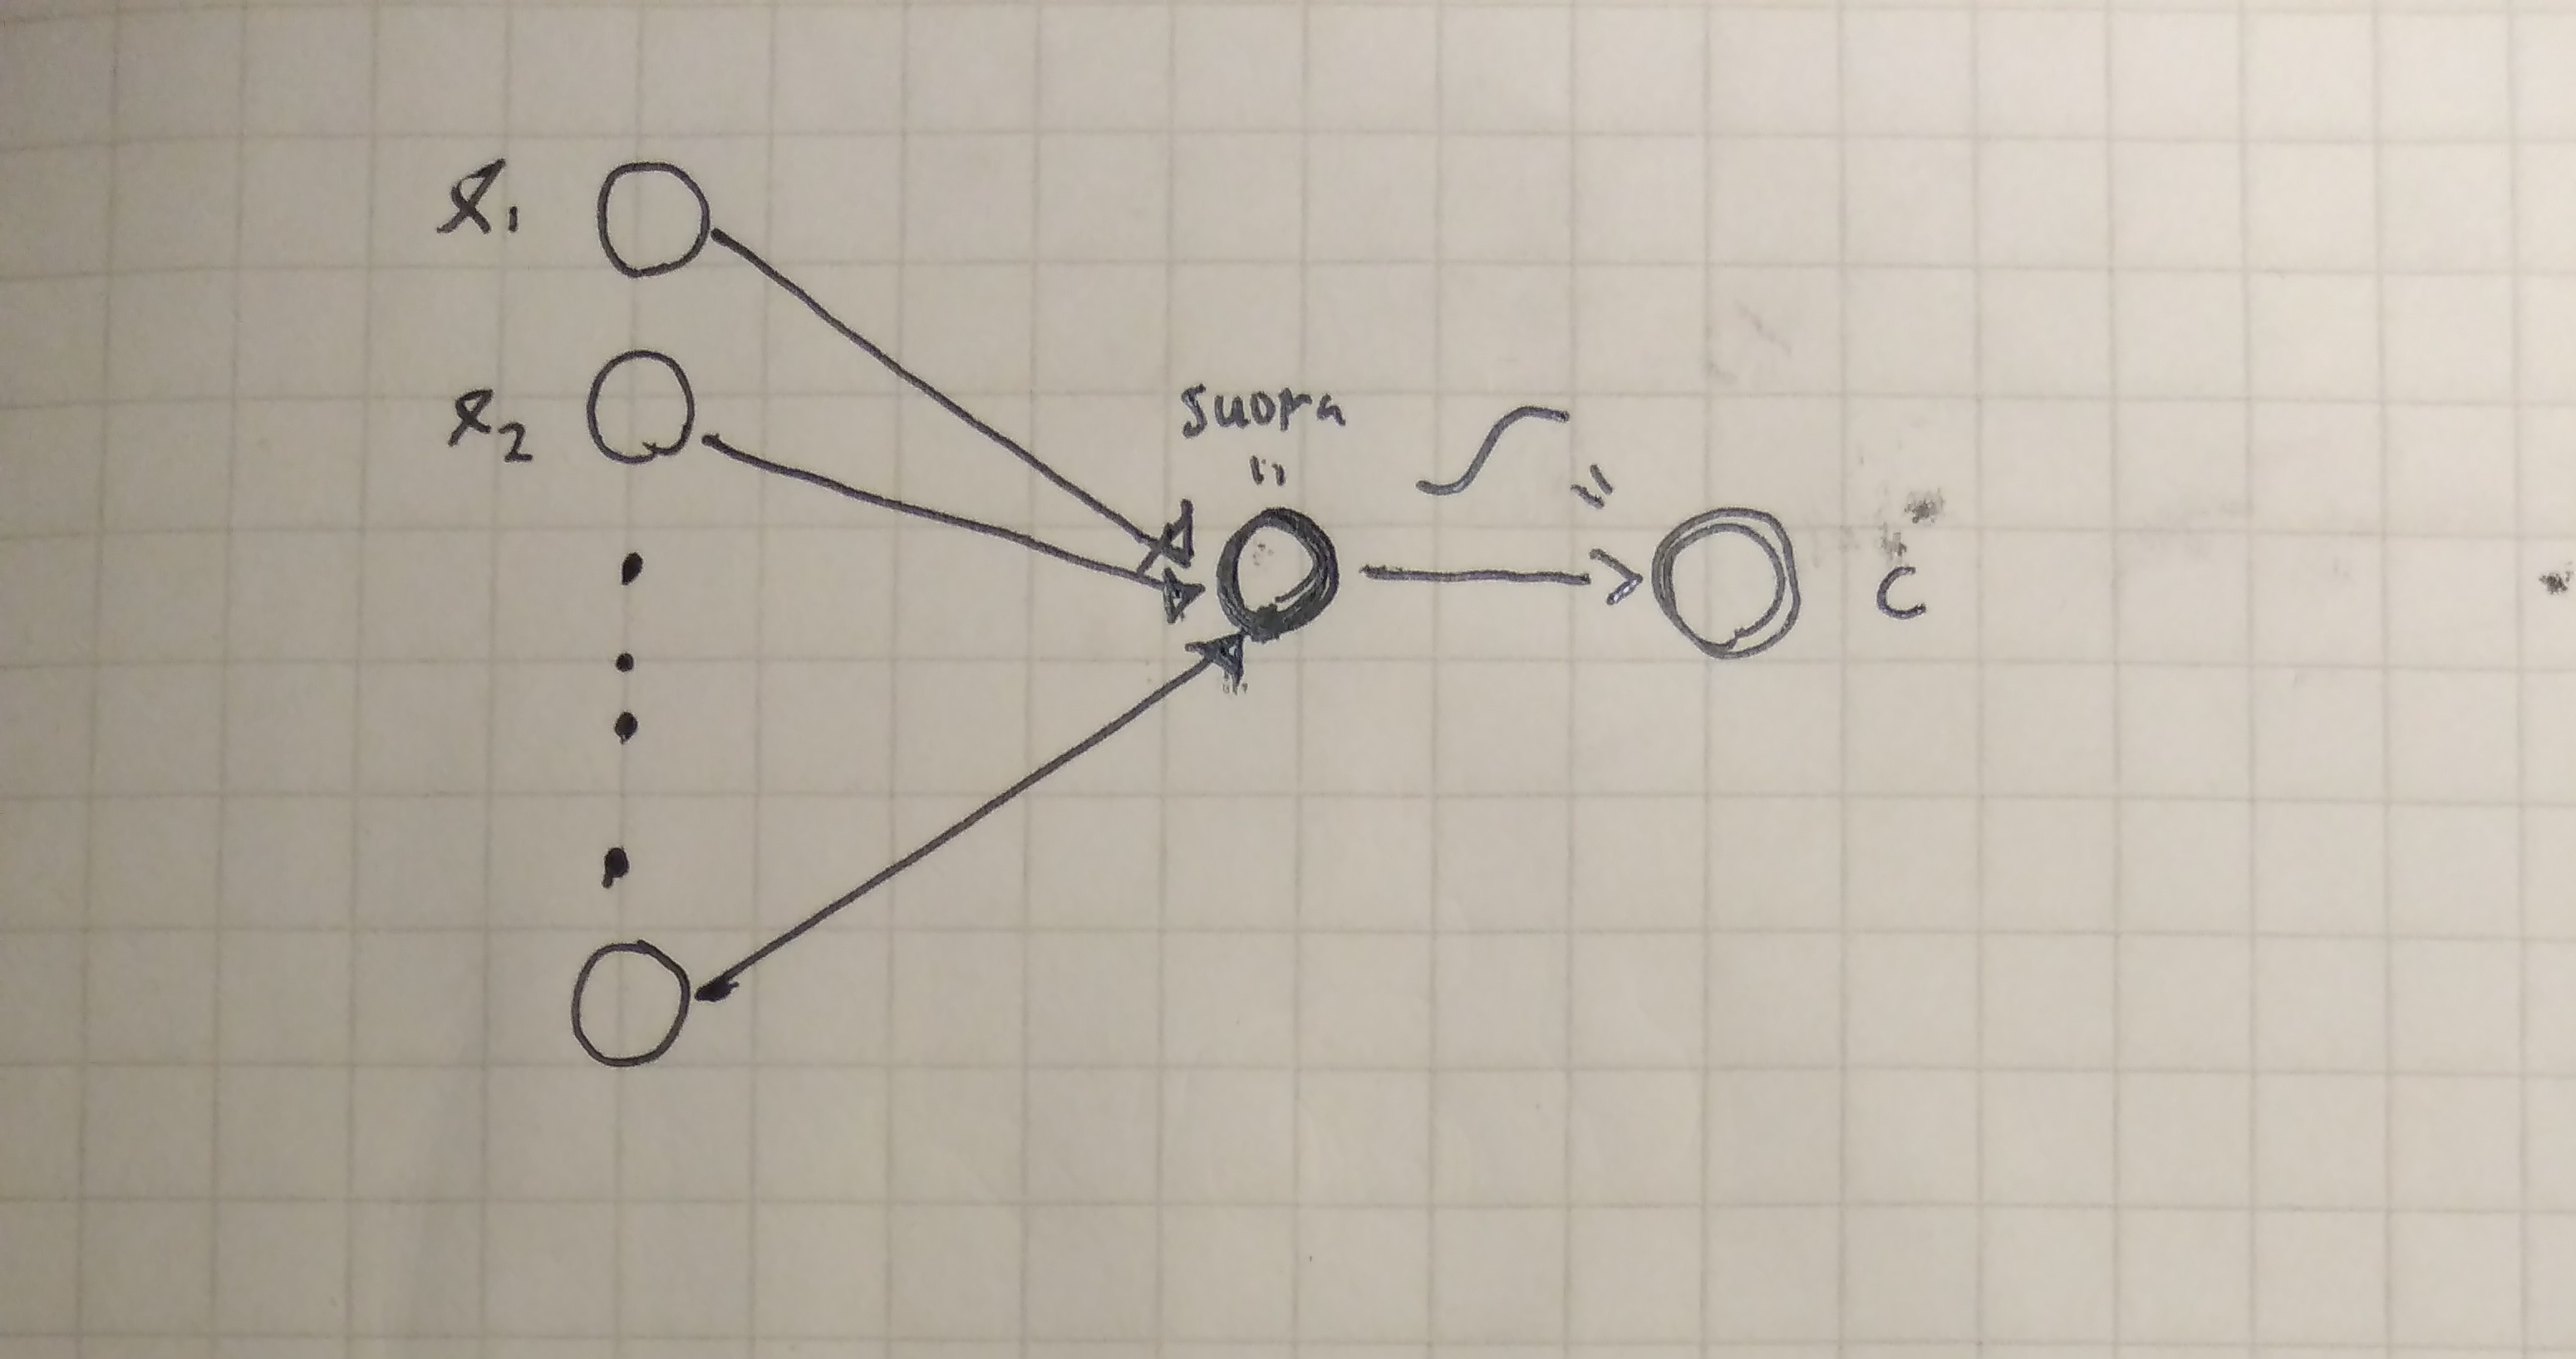
\includegraphics[width=0.8\textwidth]{logistinen_perceptron.jpg}
        
        \pause
        Logistinen regressio on neuroverkko! (Perceptron.)
\end{frame}

\begin{frame}{Hieman monimutkaisempi neuroverkko (MLP)}
    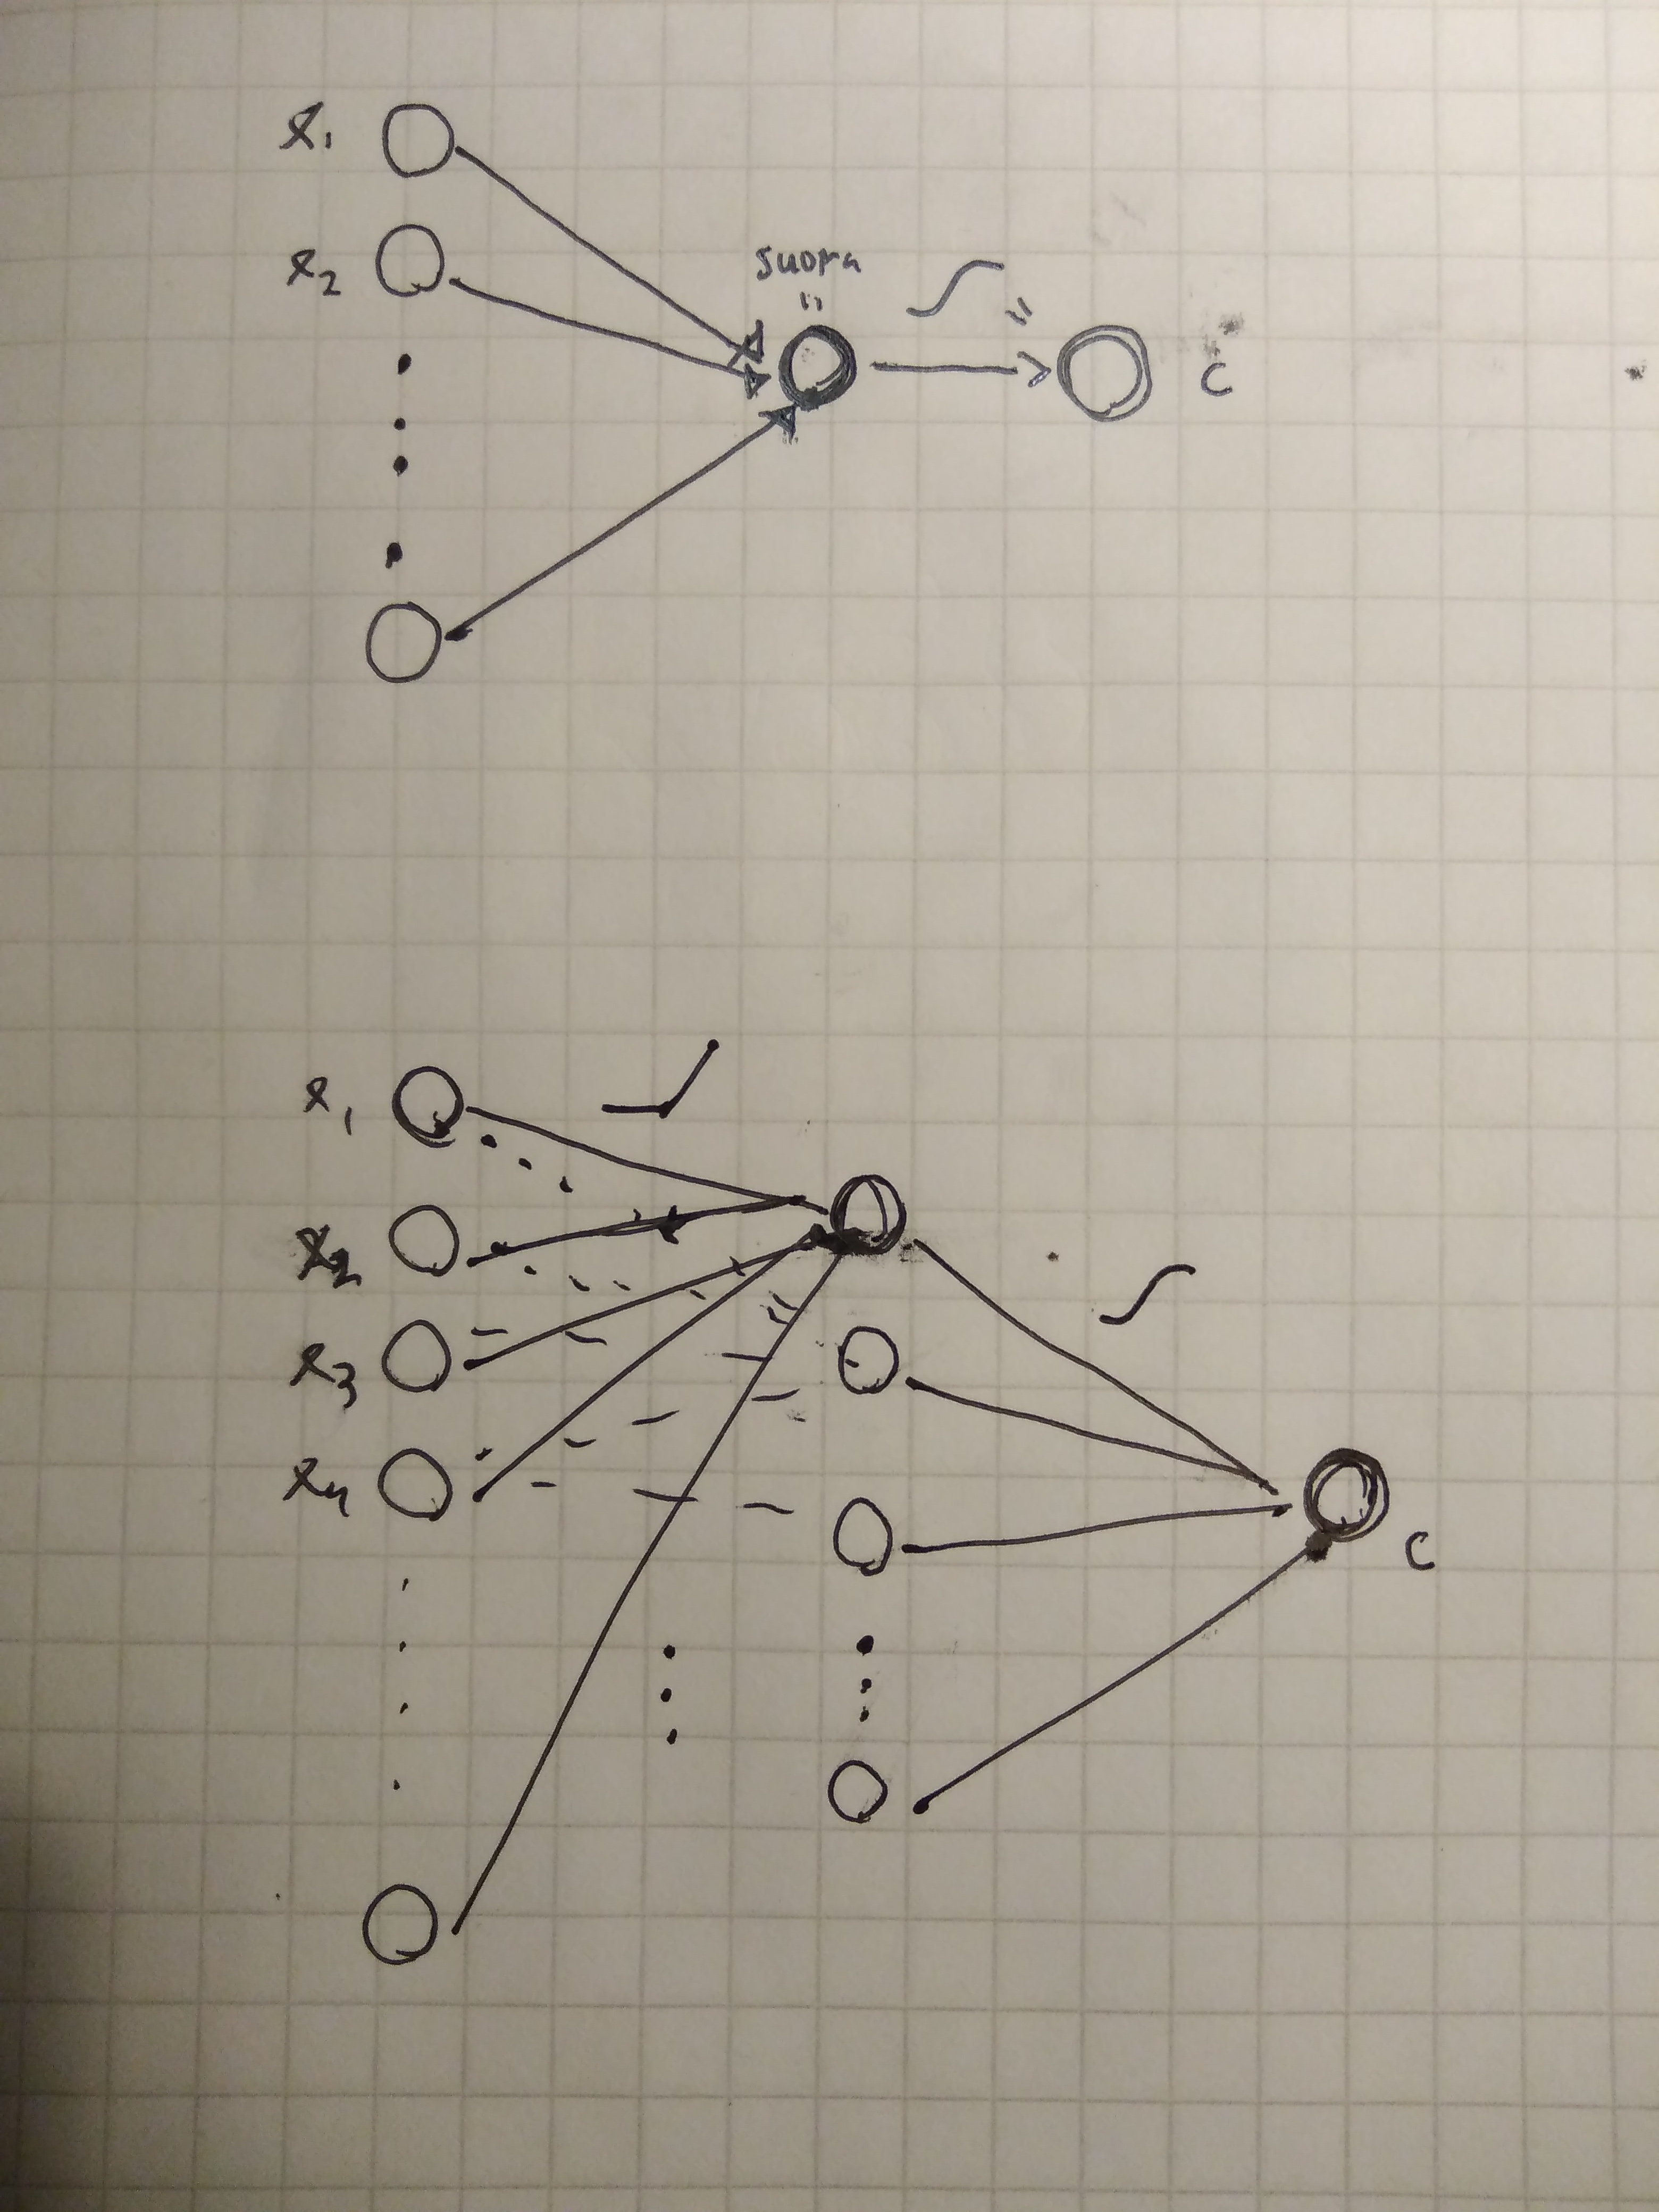
\includegraphics[width=0.5\textwidth]{mlp.jpg}
\end{frame}


\section{Kuinka eläimet selviytyvät luonnossa (MNIST-numeroiden luokittelussa)}

\begin{frame}{}
  \tableofcontents[currentsection]
\end{frame}

\begin{frame}{Miltä eläimemme näyttävät Julia-kielellä}
    	\begin{columns}[]
		\column{0.0100\textwidth}
		\column{0.4875\textwidth}
			\centering
				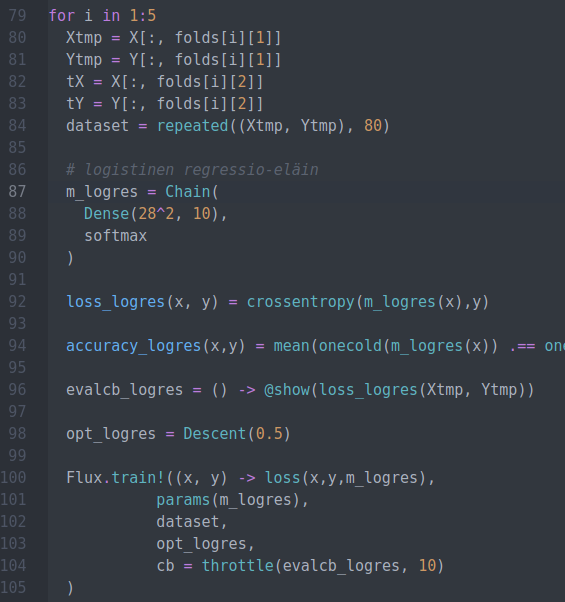
\includegraphics[width=\textwidth]{logres_elain.png}

		\column{0.4875\textwidth}
		    \centering
				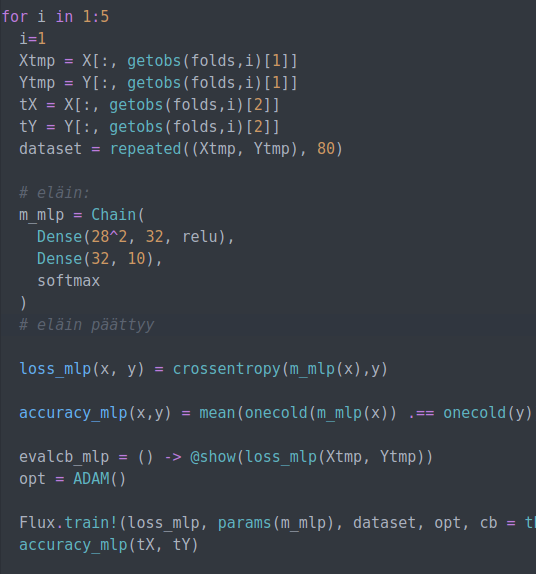
\includegraphics[width=\textwidth]{mlp_elain.png}

		\column{0.0100\textwidth}
	\end{columns}
    
\end{frame}

\begin{frame}{Kuinka eläimemme suoriutuvat numeroiden luokittelussa}

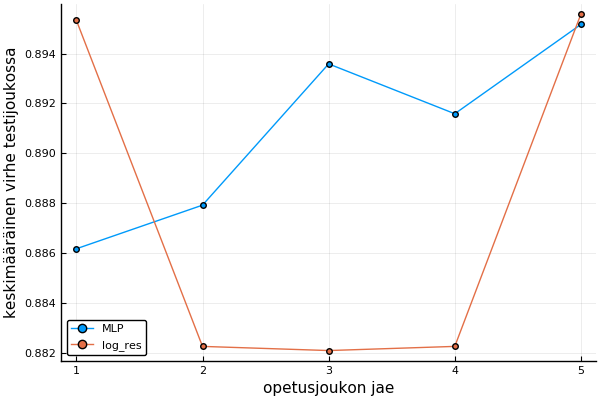
\includegraphics[width=0.7\textwidth]{mlp_logres.png}

\end{frame}

\begin{frame}{Miltä näyttää MLP-eläimen luokittelukyky}


    \begin{columns}[]
		\column{0.0100\textwidth}
		\column{0.2\textwidth}
			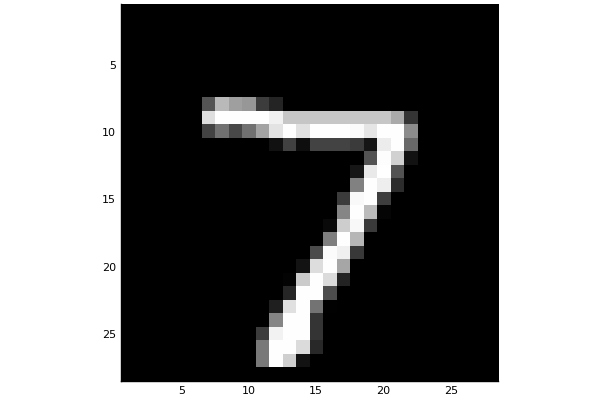
\includegraphics[width=\textwidth]{mnist1_7.png}
		\column{0.3\textwidth}
			\centering
				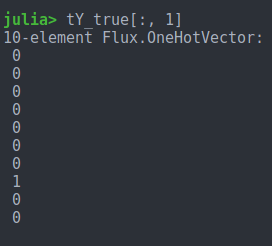
\includegraphics[width=\textwidth]{mnist_tst1_true.png}

		\column{0.3\textwidth}
		    \centering
				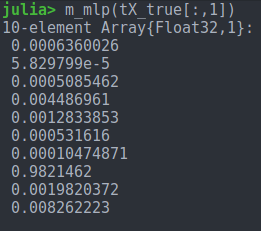
\includegraphics[width=\textwidth]{mnist_mlp_prediction.png}

		\column{0.0100\textwidth}
	\end{columns}
	\pause
	\centering
	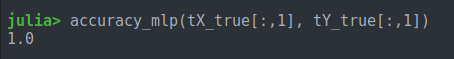
\includegraphics[width=0.6\textwidth]{accuracy.png}

\end{frame}


\begin{frame}{Lopuksi: Neuroverkkoarkkitehtuureja}

	\begin{figure}
				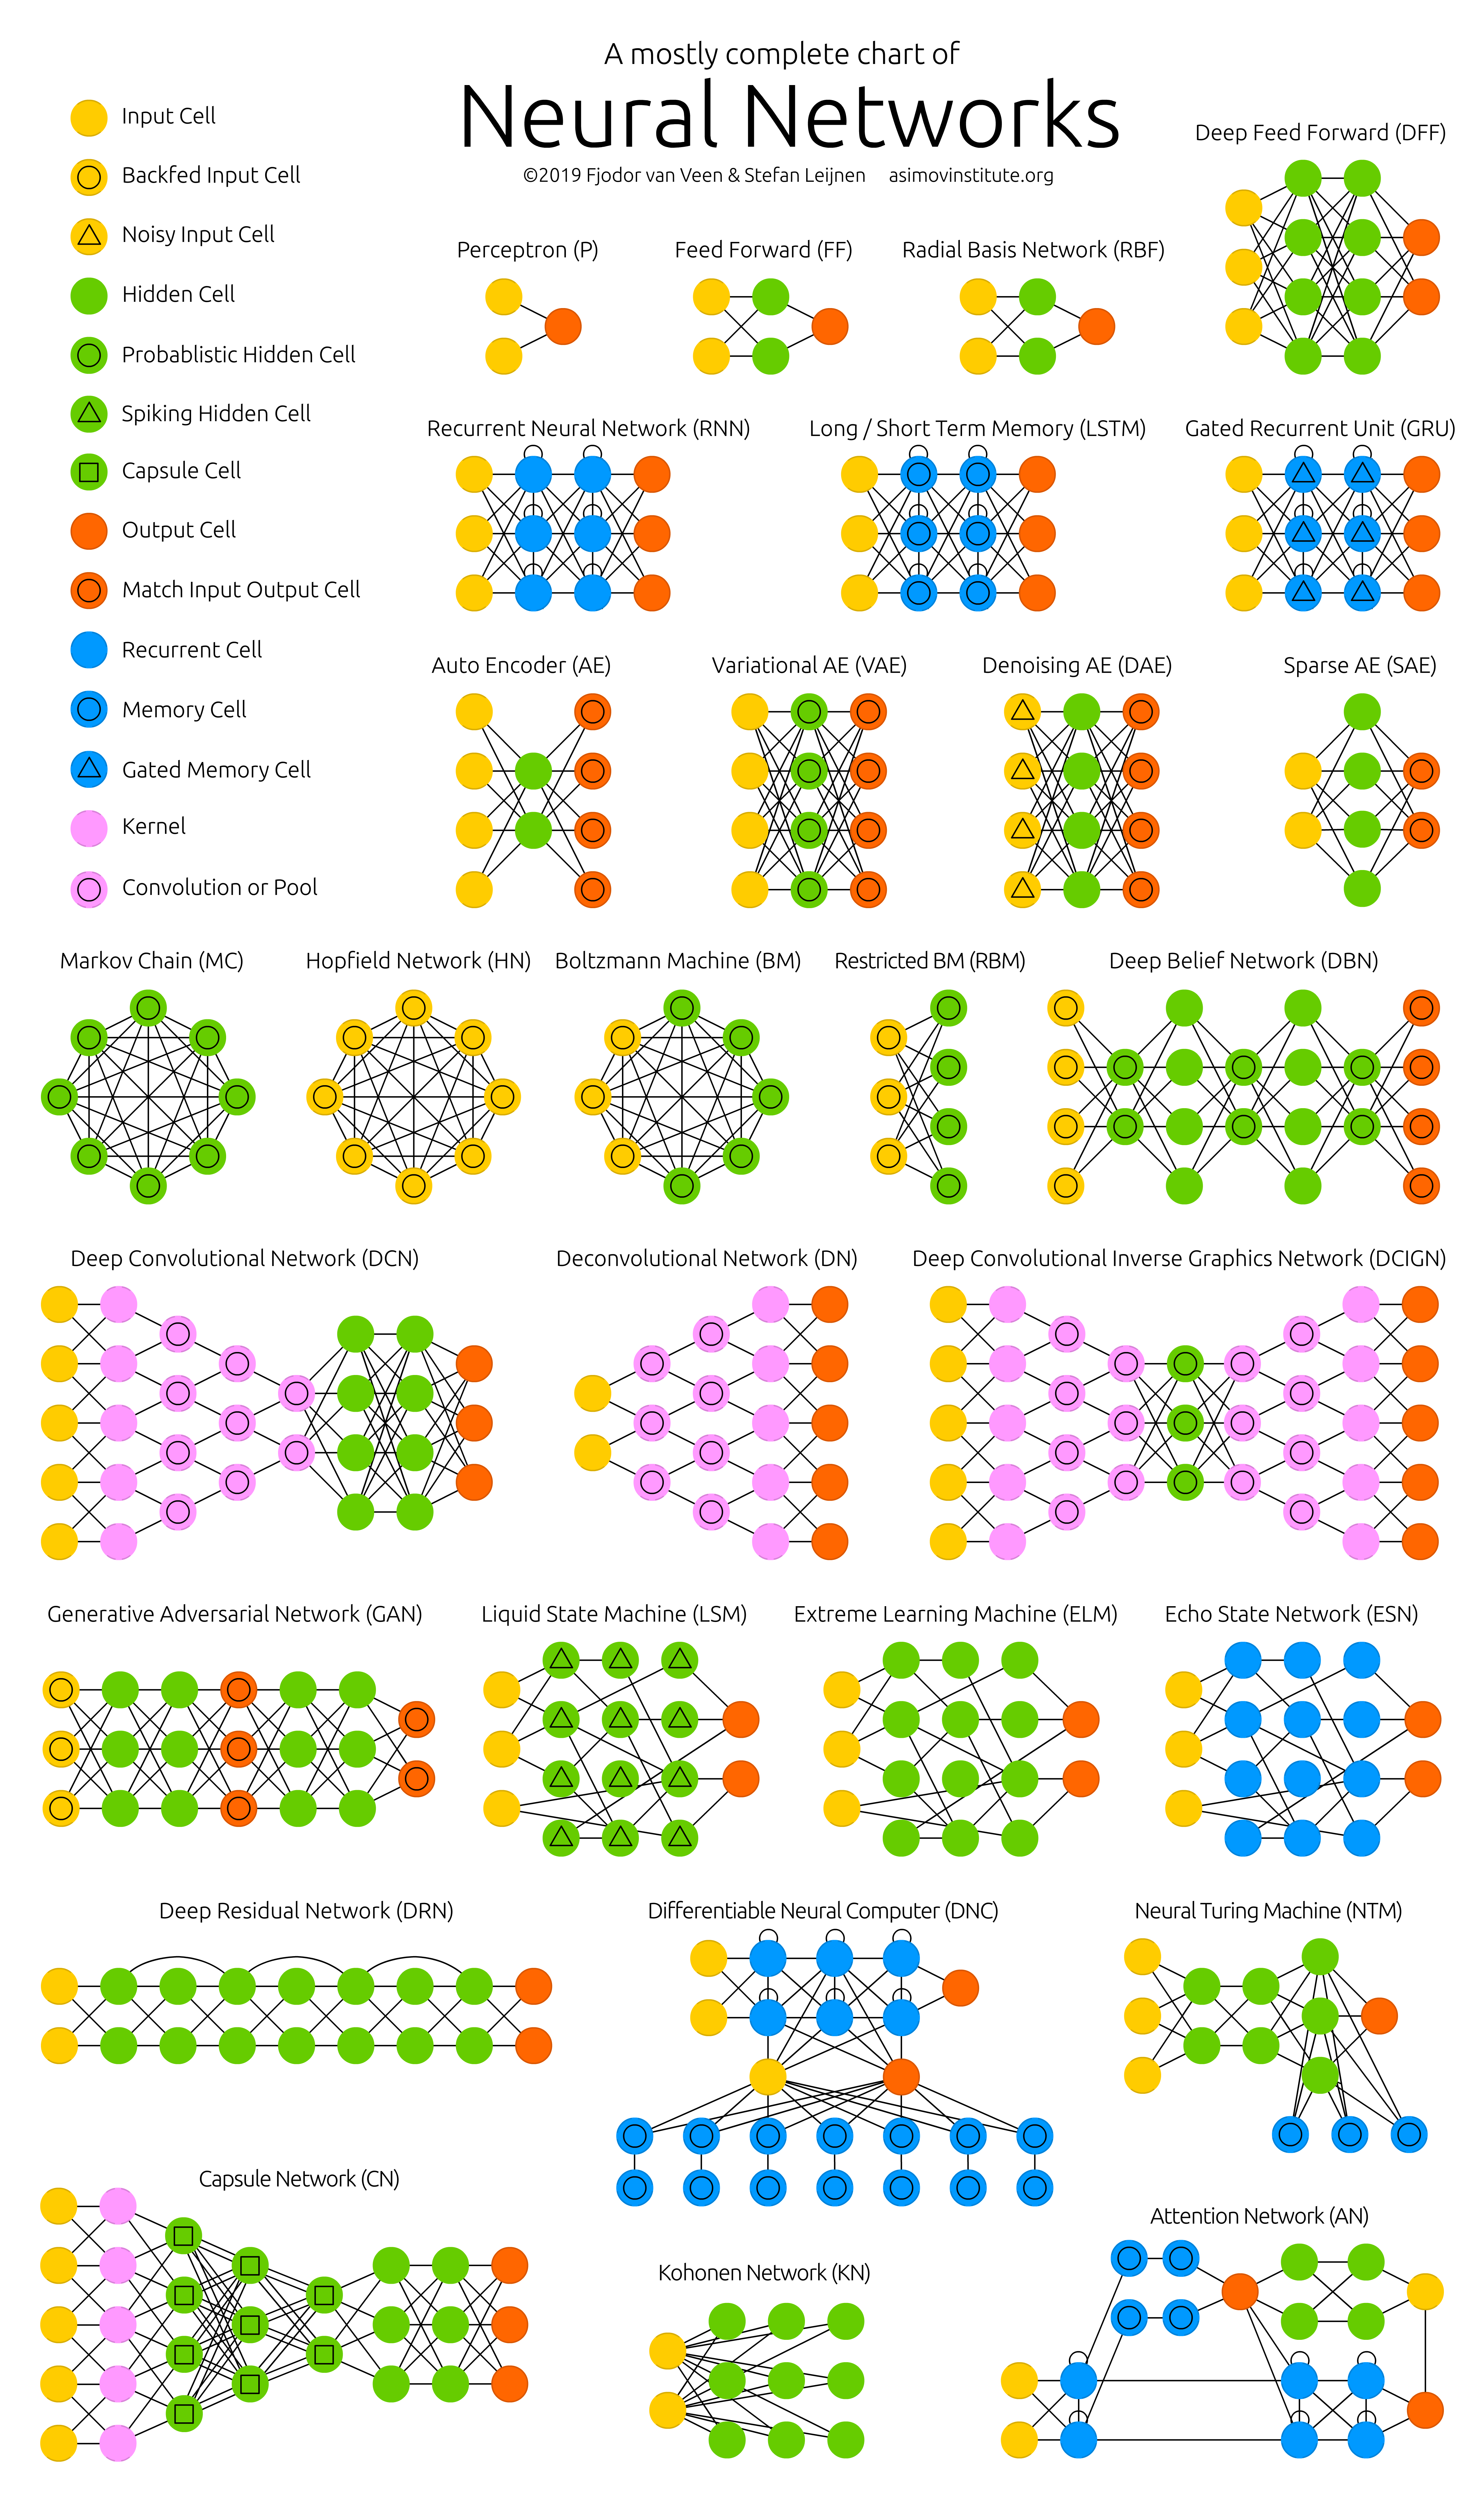
\includegraphics[height=0.65\textheight]{NeuralNetworkZo19High.png} \

				\caption*{Arkkitehtuureja on valtavasti ja kaikki tekevät erilaisia asioita hyvin, joskus. Lähde: Fjodor Van Veen, [3]}
	\end{figure}

%https://www.asimovinstitute.org/neural-network-zoo/
    
\end{frame}

%\begin{frame}{Contents}
%
%\begin{itemize}
%    \item point A
%    \item point B
%\end{itemize}
%
%\end{frame}

%\begin{frame}{Frame with lots of text}
%    \lipsum[1-1]
%\end{frame}

%\begin{frame}
%	\frametitle{Text and Figure aside}
%	\begin{columns}[]
%		\column{0.0125\textwidth}
%		\column{0.4875\textwidth}
%			\centering
%			\begin{figure}
%				%\includegraphics[draft,width=\textwidth]{fooC.pdf} \
%				% remove the 'draft' keyword, when replacing with final figure!
%				\caption{Caption of Figure C}
%			\end{figure}
%		\column{0.4875\textwidth}
%			Some text and a bullet point list
%			\begin{itemize}
%				\item ItemA
%				\item ItemB
%				\item ItemC
%				\item ItemD
%			\end{itemize}			
%		\column{0.0125\textwidth}
%	\end{columns}
%\end{frame}


\begin{frame}{Viitteitä, linkkejä ja kirjallisuutta}

    {\footnotesize
    [1] \texttt{https://commons.wikimedia.org/wiki/File:Sorting\_quicksort\_anim.gif}
    
    [2] \texttt{https://en.wikipedia.org/wiki/File:K-fold\_cross\_validation\_EN.svg}
    
    [3] \texttt{https://www.asimovinstitute.org/neural-network-zoo/}

    
    Tekoälyn perusteet (Elements of AI)-verkkokurssi:  \href{https://www.elementsofai.com/fi/}{https://www.elementsofai.com/fi/} 
    \begin{itemize}
        \item Tietääkseni keskimäärin pätevä johdanto joka on kirjoitettu ns tavalliselle kansalaiselle, mutta prof. Roosilla on vahvoja mielipiteitä siitä mikä on tulevaisuudessa mahdollista.
    \end{itemize}
    
    Richard McElreath, 2018, Statistical Rethinking. \href{https://xcelab.net/rm/statistical-rethinking/}{https://xcelab.net/rm/statistical-rethinking/}.
    \begin{itemize}
        \item Antropologin kirjoittama johdanto moderniin tilastotieteeseen, myös sen vaikeisiin osiin, joka kattaa paljon kaikenlaista paitsi neuroverkkoja (mutta antaa pohjan niiden ymmärtämiseen).
    \end{itemize}
    

    }
\end{frame}
    
\begin{frame}{Viitteitä, linkkejä ja kirjallisuutta (2)}

    Michael Nielsen, 2015, Neural Networks and Deep Learning. \href{http://neuralnetworksanddeeplearning.com/}{http://neuralnetworksanddeeplearning.com/}
    \begin{itemize}
        \item Vapaasti luettava internet-kirja neuroverkkojen perusteista.
    \end{itemize}
    
    Efron & Hastie, 2016, Computer Age Statistical Inference. \href{https://web.stanford.edu/~hastie/CASI/}{https://web.stanford.edu/~hastie/CASI/}
    \begin{itemize}
        \item Kattava oppikirja tilastollisista menetelmistä hieman edistyneemmille, jossa menetelmät selitetään ja käsittelyjärjestys seuraa historiallista kehitystä tilastotieteestä nykyaikaiseen koneoppimiseen.
    \end{itemize}
    
    Goodfellow, Bengio, Courville. 2016. Deep learning \href{http://www.deeplearningbook.org/}{http://www.deeplearningbook.org/}
    \begin{itemize}
        \item Syvien neuroverkkojen perusoppikirja edistyneille. Viime vuosien kehitystä tosin ei mukana.
    \end{itemize}

\end{frame}

\end{document}

